\documentclass[12pt]{article}
\usepackage[utf8]{inputenc}
\usepackage[T1]{fontenc}
\usepackage[vietnamese]{babel}
\usepackage{geometry}
\usepackage{amsmath}
\usepackage{anyfontsize}
\usepackage{tikz}
\usepackage{graphicx}
\usepackage{eso-pic}
\usepackage{adjustbox}
\usepackage{fancyhdr}
\usepackage{tocloft}
\usepackage{titlesec}
\usepackage{titletoc}
\usepackage{enumitem}
\usepackage{fontawesome5}
\usepackage{tabularx}
\usepackage{xcolor}
\usepackage{colortbl}
\usepackage{makecell}
\usepackage{multirow}
\usepackage{ltablex}
\usepackage{amssymb}
\usepackage{changepage}
\usepackage{hyperref}

\geometry{
    a4paper,
    left=30mm,
    right=30mm,
    top=20mm,
    bottom=20mm,
}

\pagestyle{fancy}
\fancyhf{}
\rfoot{}
\cfoot{\thepage}
\renewcommand{\headrulewidth}{0pt}
\renewcommand{\footrulewidth}{0pt}

% Tùy chỉnh mục lục với gói lệnh tocloft
\renewcommand{\cftsecleader}{\cftdotfill{\cftdotsep}}
\renewcommand{\cftsecfont}{\bfseries}
\renewcommand{\cfttoctitlefont}{\hfill\Large\bfseries}
\renewcommand{\cftaftertoctitle}{\hfill}
\renewcommand{\thepart}{PHẦN \Roman{part}.} % Định dạng phần bằng số La Mã
\renewcommand{\thesection}{\Roman{section}.} % Định dạng section bằng số La Mã
\renewcommand{\thesubsection}{\arabic{subsection}.} % Định dạng subsection bằng số
\renewcommand{\thesubsubsection}{\arabic{subsection}.\arabic{subsubsection}.} % Định dạng subsubsection bằng số

% Tùy chỉnh part
\titleformat{\part}[block]
  {\normalfont\fontsize{17}{20}\selectfont\bfseries\filright}{\thepart}{0.5em}{}
% Tùy chỉnh section
\titleformat{\section}
  {\normalfont\Large\bfseries}{\thesection}{0.5em}{}

% Tùy chỉnh subsection
\titleformat{\subsection}
  {\normalfont\large\bfseries}{\thesubsection}{0.5em}{}

% Tùy chỉnh subsubsection
\titleformat{\subsubsection}
  {\normalfont\normalsize\bfseries}{\thesubsubsection}{0.5em}{}
  
\begin{document}

\begin{titlepage}
    \centering
    
    \AddToShipoutPictureBG*{%
        \begin{tikzpicture}[remember picture, overlay]
            \node at (current page.center) {
\includegraphics[width=17cm,height=27cm]{khung.jpg}};
        \end{tikzpicture}%
    }

    \vspace*{2cm}

    \textbf{\fontsize{18}{22}\selectfont TRƯỜNG ĐẠI HỌC THỦY LỢI} \par
    \textbf{\fontsize{16}{20}\selectfont KHOA CÔNG NGHỆ THÔNG TIN} \par

    \vspace{0.5cm}
    
    \textbf{------------------------} \par

    \vspace{0.5cm}
    
    
\includegraphics[width=5cm]{Logo-Thuy_Loi.png}
    
    \vspace{0.5cm}
    
    \textbf{\fontsize{14}{18}\selectfont BÁO CÁO BÀI TẬP LỚN MÔN HỌC} \par
    \textbf{\fontsize{14}{18}\selectfont QUẢN LÝ DỰ ÁN CÔNG NGHỆ THÔNG TIN} \par
    
    \vspace{1cm}
    
    \textbf{\textit{\fontsize{12}{16}\selectfont Đề tài: QUẢN LÝ DỰ ÁN XÂY DỰNG WEBSITE}} \par
    \textbf{\textit{\fontsize{12}{16}\selectfont BÁN VÉ SỰ KIỆN TICKET FUSION}} \par
    
    \vspace{2cm}
    
    \begin{minipage}{0.4\textwidth}
        \textbf{\fontsize{10}{14}\selectfont Nhóm sinh viên thực hiện:} \par
        \vspace{2.5cm}
        \textbf{\fontsize{10}{14}\selectfont Giảng viên phụ trách môn học:}
    \end{minipage}%
    \begin{minipage}{0.25\textwidth}
        \raggedleft
        \begin{tabular}{l}
            \text{\fontsize{10}{14}\selectfont Nguyễn Ngọc Bách} \\
            \text{\fontsize{10}{14}\selectfont Nguyễn Đức Anh} \\
            \text{\fontsize{10}{14}\selectfont Nguyễn Đức Minh} \\
            \text{\fontsize{10}{14}\selectfont Trương Quốc Bảo} \\
            \text{\fontsize{10}{14}\selectfont Phạm Quỳnh Anh} \\ 
            \\
            \text{\fontsize{10}{14}\selectfont Tiến sĩ Trần Hồng Điệp}
        \end{tabular}
    \end{minipage}
    
    \vspace{3cm}
    
    \text{\fontsize{8}{12}\selectfont Hà Nội, tháng 10 năm 2023} \par
    
\end{titlepage}

\newpage
\tableofcontents
\newpage

\begin{center}
    \textbf{\fontsize{16}{20}\selectfont PHÂN CHIA CÔNG VIỆC} \par
    \vspace{2cm}
    \begin{tabular*}{\linewidth}{|>{\centering\arraybackslash}p{2cm}|>
    {\centering\arraybackslash}p{2.5cm}|>{\raggedright\arraybackslash}p{9.15cm}|}
        \hline
        \cellcolor[HTML]{C6D9F1}\rule{0pt}{1cm}\vspace{0.5cm}\textbf{Họ tên} & \cellcolor[HTML]{C6D9F1}\textbf{MSV} & \cellcolor[HTML]{C6D9F1}\makecell{\textbf{Công việc}} \\
        \hline
        \rule{0pt}{0.6cm}{Nguyễn Ngọc Bách \vspace{-3cm}}  & 2151163668 & 
        \hspace{0.2cm}- Nhóm trưởng, phân công công việc và kiểm tra\par
        \hspace{0.2cm}- Lời nói đầu\par
        \hspace{0.2cm}- Phần I. I. Giới thiệu về dự án\par
        \hspace{0.2cm}- Phần II. II. 1. Cấu trúc phân rã công việc\par
        \hspace{0.2cm}- Làm latex và PowerPoint các phần trên\par
        \hspace{0.2cm}- Thiết kế giao diện\par
        \vspace{0.2cm}
        \\
        \hline
        
        \rule{0pt}{0.6cm}{Nguyễn Đức Anh \vspace{0.3cm}} & 2151163664 &  
        \hspace{0.2cm}- Thu thập dữ liệu \par
        \hspace{0.2cm}- Phần I. II. Mục tiêu dự án\par
        \hspace{0.2cm}- Phần II. II. 4. Quản lý chi phí\par
        \hspace{0.2cm}- Làm latex và PowerPoint các phần trên\par
        \hspace{0.2cm}- Thiết kế giao diện\par
        \vspace{0.2cm}
        \\
        \hline

        \rule{0pt}{0.6cm}{Nguyễn Đức Minh \vspace{0.3cm}} & 2151163707 & 
        \hspace{0.2cm}- Thu thập dữ liệu \par
        \hspace{0.2cm}- Phần I. III. Thiết lập môi trường dự án \par
        \hspace{0.2cm}- Phần II. II. 3. Quản lý thời gian\par
        \hspace{0.2cm}- Làm latex và PowerPoint các phần trên\par
        \hspace{0.2cm}- Thiết kế giao diện\par
        \vspace{0.2cm}
        \\
        \hline

        \rule{0pt}{0.6cm}{Trương Quốc Bảo \vspace{0.3cm}} & 2151163669 &  
        \hspace{0.2cm}- Phần II. I. Kế hoạch tổng thể  \par
        \hspace{0.2cm}- Phần II. II. 2. Quản lý phạm vi\par
        \hspace{0.2cm}- Phần III. CHUYỂN GIAO\par
        \hspace{0.2cm}- Làm latex và PowerPoint các phần trên\par
        \hspace{0.2cm}- Thiết kế giao diện\par
        \vspace{0.2cm}
        \\
        \hline

        \rule{0pt}{0.6cm}{Phạm Quỳnh Anh \vspace{0.3cm}} & 2151160530 & 
        \hspace{0.2cm}- Phần II. II. 5. Quản lý chất lượng\par
        \hspace{0.2cm}- Phần II. II. 6. Quản lý nguồn nhân lực\par
        \hspace{0.2cm}- Phần IV. KẾT LUẬN \par
        \hspace{0.2cm}- Làm latex và PowerPoint các phần trên \par
        \hspace{0.2cm}- Làm kịch bản và thuyết trình \par
        \vspace{0.2cm}
        \\
        \hline
    \end{tabular*}
\end{center} 

\clearpage

\begin{center}
    \textbf{\fontsize{16}{20}\selectfont LỜI NÓI ĐẦU} \par
\end{center}
\vspace{2cm}
\hspace{1cm}Trong thời đại hiện đại, công nghệ thông tin đã trở thành một phần không thể thiếu của cuộc sống hàng ngày. Các tiến bộ trong lĩnh vực này đã mở ra những cánh cửa mới, tạo nên sự kết nối và tiện lợi chưa từng có trước đây. Internet đã trở thành một mạng lưới toàn cầu, kết nối mọi người từ khắp nơi trên thế giới. Điện thoại di động đã trở thành một tiện ích không thể thiếu, mang đến khả năng liên lạc và truy cập thông tin mọi lúc, mọi nơi. Công nghệ trí tuệ nhân tạo và học máy đang ngày càng phát triển, mang lại những khả năng tính toán và phân tích thông tin vượt trội. Trong bối cảnh này, hệ thống bán vé trực tuyến Ticket Fusion đã nổi lên như một giải pháp tiên tiến và đáng chú ý. Với sự phát triển mạnh mẽ của công nghệ và sự phổ biến của mua sắm trực tuyến, việc mua vé trực tuyến đã trở thành một xu hướng phổ biến. Người dùng muốn có thể dễ dàng tìm hiểu về các sự kiện, lựa chọn và mua vé một cách nhanh chóng và an toàn. Ticket Fusion xuất hiện để đáp ứng nhu cầu này và tận dụng các tiến bộ công nghệ để mang lại trải nghiệm mua vé tuyệt vời. Với sự phát triển nhanh chóng của công nghệ thông tin và sự lan truyền rộng rãi của Internet, việc tận dụng công nghệ để cung cấp dịch vụ trực tuyến trở nên ngày càng quan trọng và phổ biến. Ticket Fusion đã tận dụng tối đa những tiềm năng đó và xây dựng một hệ thống bán vé trực tuyến đáng tin cậy, tiện lợi và hấp dẫn.

\newpage

\part{KHỞI ĐỘNG DỰ ÁN}

\section{Giới thiệu về dự án}

\subsection{Tên dự án}
\hspace{1cm}- Xây dựng Website bán vé sự kiện \textbf{TicketFusion}

\subsection{Trưởng nhóm dự án}
\hspace{1cm}- Nguyễn Ngọc Bách

\subsection{Thành viên tổ dự án}
\hspace{1cm}- Tổ dự án gồm 5 thành viên:
\begin{itemize}[label=+, leftmargin=2cm]
\item Nguyễn Ngọc Bách
\item Nguyễn Đức Anh
\item Phạm Quỳnh Anh
\item Trương Quốc Bảo
\item Nguyễn Đức Minh
\end{itemize}

\subsection{Chủ đầu tư kiêm khách hàng}
\begin{itemize}[label=, leftmargin=1cm]
\item Công ty TNHH MTV Hồng Diệp (shop bán vé Hồng Diệp)
\item Đại diện: Bà Trần Hồng Diệp
\item Địa chỉ: 175 Tây Sơn, Đống Đa, Hà Nội
\item Số điện thoại: 0969696969
\item Email: shophongdiep@gmail.com
\end{itemize}

\subsection{Cơ quan chủ quản thực hiện dự án}
\begin{itemize}[label=, leftmargin=1cm]
\item Công ty Cổ phần Công nghệ BBB
\item Đại diện: Nguyễn Ngọc Bách
\item Địa chỉ: 520 Tây Sơn, Đống Đa, Hà Nội
\item Số điện thoại: 0829922785
\item Email: bach01299929715@gmail.com
\end{itemize}

\section{Mục tiêu dự án}

\subsection{Mục tiêu doanh nghiệp}
\begin{itemize}[label=-, leftmargin=1cm]
\item Tạo ra một giao diện người dùng trực tuyến dễ sử dụng và thân thiện, nhằm giúp người dùng mua vé một cách thuận tiện và nhanh chóng.
\item Cung cấp một giao diện quản lý sự kiện dễ sử dụng cho người quản lý, cho phép tạo mới sự kiện, quản lý thông tin vé, định rõ chính sách hoàn vé và tạo mô phỏng hội trường.
\item Đảm bảo tính an toàn và tiện lợi bằng cách tích hợp các hệ thống thanh toán an toàn, giúp người dùng thực hiện thanh toán một cách dễ dàng và bảo mật.
\item Xây dựng mạng lưới đối tác và nhà cung cấp vé đáng tin cậy và đa dạng, nhằm mang đến cho người dùng một loạt các sự kiện và vé khác nhau.
\item Cung cấp các kênh tương tác và hỗ trợ khách hàng, bao gồm trò chuyện trực tuyến, email và số điện thoại, để đảm bảo sự hỗ trợ nhanh chóng và tận tâm khi cần thiết.
\item Tạo ra các chiến dịch tiếp thị và quảng cáo hiệu quả, nhằm tăng doanh số bán hàng và doanh thu của nền tảng.
\item Thu thập và phân tích dữ liệu để theo dõi và đánh giá hiệu suất của nền tảng, từ đó cải thiện các chỉ số quan trọng như doanh số bán hàng, tỷ lệ chuyển đổi và khách hàng trung thành.
\item Xây dựng một thương hiệu mạnh mẽ và đáng tin cậy bằng cách cung cấp dịch vụ chất lượng cao, chăm sóc khách hàng tốt và xây dựng mối quan hệ lâu dài với khách hàng.
\end{itemize}

\subsection{Mục tiêu công nghệ}
\begin{itemize}[label=-, leftmargin=1cm]
\item Phát triển một giao diện người dùng hấp dẫn và thân thiện: Mục tiêu của chúng tôi là tạo ra một giao diện người dùng đẹp mắt, dễ sử dụng và thân thiện. Điều này đòi hỏi áp dụng các nguyên tắc thiết kế tốt, tối ưu hóa trải nghiệm người dùng và cung cấp các chức năng dễ tiếp cận. Giao diện người dùng cần tương thích với nhiều thiết bị và trình duyệt khác nhau để đáp ứng nhu cầu của người dùng.
\item Xây dựng hệ thống quản lý cơ sở dữ liệu hiệu quả: Mục tiêu của chúng tôi là xây dựng một hệ thống quản lý cơ sở dữ liệu (Database Management System - DBMS) hiệu quả. Hệ thống này sẽ được sử dụng để lưu trữ và quản lý thông tin về sự kiện, vé, khách hàng và các giao dịch liên quan. Chúng tôi sẽ tập trung vào tính nhất quán của dữ liệu, bảo mật thông tin và khả năng mở rộng để đáp ứng nhu cầu xử lý lượng dữ liệu lớn và mở rộng khi cần thiết.
\item Tối ưu hóa hiệu suất và tải trang: Mục tiêu là tối ưu hóa hiệu suất và thời gian tải trang của website. Chúng tôi sẽ sử dụng các kỹ thuật tối ưu hóa mã nguồn, bộ nhớ cache và tải nội dung theo yêu cầu để cải thiện trải nghiệm người dùng và giảm thời gian phản hồi.
\item Đảm bảo tính bảo mật của hệ thống: Mục tiêu quan trọng là đảm bảo tính bảo mật của hệ thống để bảo vệ thông tin cá nhân và giao dịch của khách hàng. Chúng tôi sẽ triển khai các biện pháp bảo mật vượt trội như mã hóa dữ liệu, xác thực hai bước và giám sát hệ thống để phát hiện và ngăn chặn các mối đe dọa tiềm ẩn.
\item Tích hợp các phương thức thanh toán trực tuyến: Mục tiêu là tích hợp các phương thức thanh toán trực tuyến như thẻ tín dụng, ví điện tử và các cổng thanh toán khác vào website. Điều này đảm bảo rằng khách hàng có nhiều lựa chọn thanh toán và giao dịch an toàn và thuận tiện.
\item Đảm bảo khả năng mở rộng và linh hoạt: Mục tiêu là xây dựng một hệ thống có khả năng mở rộng và linh hoạt để đáp ứng nhu cầu tăng trưởng của doanh nghiệp. Chúng tôi sẽ sử dụng kiến trúc mô-đun, phân tách chức năng và sử dụng công nghệ có khả năng mở rộng để dễ dàng mở rộng hệ thống khi cần thiết.
\end{itemize}

\subsection{Các điều kiện ràng buộc}
\begin{itemize}[label=-, leftmargin=1cm]
\item Mọi rủi ro về mặt kỹ thuật, con người thì khách hàng không chịu trách nhiệm.
\item Nếu có lỗi trong thời gian bảo trì thì phía bên nhóm sẽ được bên doanh nghiệp hỗ trợ tùy tình huống thì nhóm sẽ có thể phải chịu toàn bộ trách nhiệm.
\item Sau khi hoàn thành dự án nhóm phải xóa toàn bộ dữ liệu trên máy của nhóm bàn giao mọi thứ lại cho khách hàng, việc bảo trì và nâng cấp khách hàng sẽ cung cấp lại dữ liệu sau cho nhóm để đảm bảo nhóm không lợi dụng sản phẩm.
\item Phía khách hàng không chấp nhận nếu sản phẩm chậm 15 ngày, sản phẩm không đảm bảo chất lượng, không đúng yêu cầu.
\item Khi sản phẩm cần nâng cấp thì khách hàng sẽ chi them chi phí cho nhóm.
\end{itemize}
\newpage
\subsection{Tôn chỉ dự án}
\keepXColumns
\begin{tabularx}{\textwidth}{|>{\raggedright\arraybackslash}X|}
    \hline
    {\cellcolor[HTML]{6D9EEB}\textbf{\rule{0pt}{1cm}\makecell{\ TÔN CHỈ DỰ ÁN (PROJECT CHARTER) \vspace{0.5cm}}}} \\
    \hline
    \multicolumn{1}{|p{\dimexpr\linewidth-0.5cm-2\tabcolsep}|}{%
    \begin{itemize}[label=, leftmargin=0.5cm]
        \item \textbf{Tên dự án:} Xây dựng Website mua bán vé sự kiện \textbf{(TicketFusion)}
        \item \textbf{Nhà đầu tư (Bên A):} Công Ty TNHH MTV Hồng Diệp
        \item \textbf{Ngày bắt đầu:} 04/09/2023
        \item \textbf{Ngày kết thúc:} 30/11/2023
        \item \textbf{Ngân sách:} 150.000.000 VND
        \item \textbf{Mục tiêu dự án:}
            \begin{itemize}[label=-, leftmargin=1cm]
            \item Mục tiêu dự án là xây dựng một nền tảng website mua bán vé trực tuyến đáng tin cậy và tiện lợi cho Công Ty TNHH MTV Hồng Diệp. Chúng tôi cam kết đảm bảo trải nghiệm mua vé dễ dàng cho khách hàng và cung cấp giao diện quản lý sự kiện thuận tiện cho người quản lý sự kiện.
            \end{itemize}
        \item \textbf{Chức năng nghiệp vụ:}
            \begin{itemize}[label=-, leftmargin=1cm]
            \item Quản lý người dùng với các tác vụ khác nhau.
            \item Phân cấp người dùng.
            \item Cập nhật thông tin vé, sự kiện.
            \item Có thể đăng nhập bằng tài khoản Facebook hoặc Gmail.
            \item Có các chức năng như tìm kiếm, quản lý sự kiện, xem thông tin sự kiện, mua và quản lý vé,...
            \end{itemize}
        \item \textbf{Yêu cầu kỹ thuật:}
            \begin{itemize}[label=-, leftmargin=1cm]
            \item Dễ dàng nâng cấp chỉnh sửa sau này kể cả đối với một đội ngũ làm việc khác.
            \item Giao diện thân thiện với người dùng, dễ sử dụng.
            \item Hệ thống chạy mượt mà ổn định.
            \item Tương thích với nhiều Browser khác nhau.
            \item Tốc độ truy cập nhanh, chính xác cho phép nhiều người dùng truy cập sử dụng một lúc.
            \end{itemize}
        \item \textbf{Yêu cầu khác:} 
            \begin{itemize}[label=-, leftmargin=1cm]
            \item Đảm bảo tính hợp pháp, bản quyền.
            \item Bảo trì sản phẩm trong quá trình sử dụng và sửa lỗi hệ thống khi có sự cố.
            \end{itemize}
    \end{itemize}} \\
    \hline
\end{tabularx}

    \begin{tabularx}{\textwidth}{|>{\raggedright\arraybackslash}X|}
    \hline
    \multicolumn{1}{|p{\dimexpr\linewidth-2\tabcolsep}|}{%
    \begin{itemize}[label=, leftmargin=0.5cm, rightmargin=0.5cm]
        \item \hspace{0.5cm} - Hoàn thành trước ngày 25/11/2023.
        \item \textbf{Cách tiếp cận:} 
            \begin{itemize}[label=-, leftmargin=1cm]
            \item Tìm hiểu yêu cầu mà khách hàng mong muốn xây dựng phần mềm.
            \item Tìm hiểu các đối tượng sử dụng phần mềm mà khách hàng mong muốn phần mềm hướng tới để đạt được hiệu quả cao nhất.
            \item Lựa chọn ngôn ngữ phù hợp để phát triển.
            \item Đánh giá kết quả đạt được của dự án.
            \item Áp dụng mô hình thác nước để làm ra sản phẩm
            \item Sử dụng ngôn ngữ PHP để phát triển dự án.
            \item Sử dụng MySQL để lưu trữ dữ liệu.
            \item Thiết kế cơ sở dữ liệu phù hợp với các yêu cầu của dự án.
            \end{itemize}
        \item \textbf{Vai trò và ký kết:} \par
            \begin{tabular*}{\linewidth}{|>{\centering\arraybackslash}p{2cm}|>{\centering\arraybackslash}p{3cm}|>
            {\centering\arraybackslash}p{3cm}|>{\centering\arraybackslash}p{3.8cm}|}
            \hline
            \cellcolor[HTML]{C6D9F1}\rule{0pt}{1cm}\vspace{0.5cm}\textbf{Vai trò} & \cellcolor[HTML]{C6D9F1}\textbf{Họ tên} & \cellcolor[HTML]{C6D9F1}\textbf{Tổ chức/Vị trí} & \cellcolor[HTML]{C6D9F1}\textbf{Liên hệ} \\
            \hline
            \rule{0pt}{0.6cm}{Giám đốc dự án \vspace{0.3cm}} & Nguyễn Ngọc Bách & Trưởng nhóm dự án & bach01299929785 @gmail.com\\
            \hline

            \rule{0pt}{0.6cm}{\multirow{4}{2cm}{Nhóm thực hiện dự án \vspace{-3.5cm}}} & 
            \multicolumn{1}{>{\centering\arraybackslash}p{3cm}|}{Nguyễn Đức Anh \vspace{0.3cm}} & \rule{0pt}{0.6cm}{\multirow{4}{2cm}{\makecell{Nhóm 1 \vspace{-3.5cm}}}} & \multicolumn{1}{>{\centering\arraybackslash}p{3.8cm}|}{nguyenducanh 10102003@gmail.com} \\

            \cline{2-2}\cline{4-4}
            
            \rule{0pt}{0.6cm} & Trương Quốc Bảo \vspace{0.3cm} &  & \multicolumn{1}{>{\centering\arraybackslash}p{3.8cm}|}{truongquocbao63664 @gmail.com} \\

            \cline{2-2}\cline{4-4}
            
            \rule{0pt}{0.6cm} & Nguyễn Đức Minh \vspace{0.3cm} &  & \multicolumn{1}{>{\centering\arraybackslash}p{3.8cm}|}{minhyeuhau520 @gmail.co} \\

            \cline{2-2}\cline{4-4}

            \rule{0pt}{0.6cm} & Phạm Quỳnh Anh \vspace{0.3cm} &  & \multicolumn{1}{>{\centering\arraybackslash}p{3.8cm}|}{phamquanum1592k3 @gmail.com} \\
            
            \hline
            
            \rule{0pt}{0.6cm}{Khách hàng \vspace{0.3cm}} & Trần Hồng Diệp & Chủ đầu tư & shophongdiep @gmail.com\\
            \hline
            \end{tabular*}
    \end{itemize}} \\
    \vspace{0.2cm} \\
    \hline
\end{tabularx}
\newpage
\section{Thiết lập môi trường dự án}
\subsection{Hạ tầng kỹ thuật}
\hspace{1cm}- Nguyên vật liệu
\begin{itemize}[label=+, leftmargin=2cm]
\item Phí thuê máy chủ.
\item Chi phí đăng ký bản quyền tên miền.
\item Các thiết bị khác.
\item Chi phí in phiếu khảo sát.
\item Bút viết.
\item Thẻ nhớ.
\item Các đồ dùng khác.
\end{itemize}

\hspace{0.3cm}- Cơ sở vật chất
\begin{itemize}[label=+, leftmargin=2cm]
\item Chi phí thuê máy quay, máy ghi âm.
\item Chi phí điện.
\item Chi phí Internet.
\item Chi phí thuê văn phòng.
\item Chi phí phụ phát sinh.
\end{itemize}

\hspace{0.3cm}- Chi phí phát sinh
\begin{itemize}[label=+, leftmargin=2cm]
\item Chi phí đi lại gặp gỡ phỏng vấn khách hàng.
\item Chi phí đi lại khảo sát.
\item Chi phí liên lạc, điện thoại trao đổi với khách hàng.
\item Chi phí sinh hoạt văn phòng.
\item Chi phí liên hoan.
\end{itemize}

\faArrowRight \hspace{0.2cm} Các chi phí sẽ do công ty chủ quản chi trả trong quá trình hoàn thiện dự án.

\subsection{Các phần mềm sử dụng}
\begin{itemize}[label=-, leftmargin=1cm]
\item HTML, PHP, CSS, Jquery/JS, React
\item MySQL
\item StarUML
\item Figma
\item Latex
\end{itemize}

\newpage

\part{KẾ HOẠCH QUẢN LÝ}
\setcounter{section}{0}
\section{Kế hoạch tổng thể}
\subsection{Đội phát triển dự án}
\begin{tabular*}{\linewidth}{|>{\centering\arraybackslash}p{4cm}|>
{\centering\arraybackslash}p{6cm}|>{\raggedright\arraybackslash}p{3.65cm}|}
        \hline
        \cellcolor[HTML]{C6D9F1}\rule{0pt}{1cm}\vspace{0.5cm}\textbf{Vai trò} & \cellcolor[HTML]{C6D9F1}\textbf{Trách nhiệm} & \cellcolor[HTML]{C6D9F1}\makecell{\textbf{Thành viên}} \\
        \hline
        \rule{0pt}{1cm}{Quản lý dự án (Project manager) \vspace{1cm}}  & Người quyết định, đưa ra các vai  trò tham gia, các tài nguyên cho  dự án & Nguyễn Ngọc Bách
        \\
        \hline
        \rule{0pt}{1cm}{Nhân viên phân tích (Business Analyst) \vspace{1cm}}  & Phân tích các yêu cầu nghiệp vụ dựa trên những yêu cầu của khách  hàng & Nguyễn Ngọc Bách
        \\
        \hline
        \rule{0pt}{1cm}{Thiết kế (Designer) \vspace{0.5cm}}  & Phân tích thiết kế giao diện & Nguyễn Đức Minh
        \\
        \hline
        \rule{0pt}{1cm}{Kiểm thử (Tester) \vspace{1cm}}  & Chịu trách nhiệm kiểm thử hệ thống & Phạm Quỳnh Anh \par
        Trương Quốc Bảo
        \\
        \hline
        \rule{0pt}{1cm}{Kỹ thuật viên (Technical)\vspace{1cm}}  & Triển khai hệ thống khách hàng,  chịu trách nhiệm cài đặt & Nguyễn Đức Anh
        \\
        \hline
        \rule{0pt}{1cm}{Lập trình viên (Developer) \vspace{1cm}}  & Cài đặt, xây dựng và phát triển hệ thống & Phạm Quỳnh Anh \par Trương Quốc Bảo \par Nguyễn Đức Anh \par Nguyễn Đức Minh \par
        \\
        \hline
    \end{tabular*}
\newpage
\subsection{Vòng đời phát triển dự án}
\hspace{1cm}\textbf{- Mô hình thác nước}
\par
\vspace{1cm}
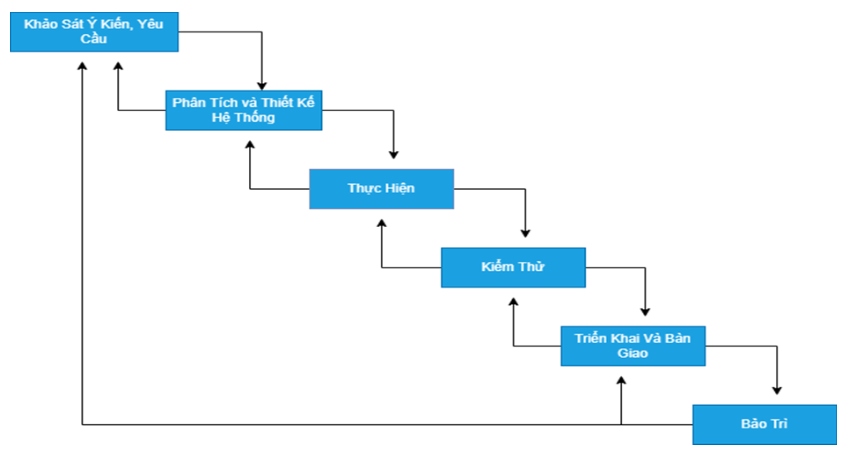
\includegraphics[width=14cm]{mo_hinh_thac_nuoc.png}
\vspace{1cm}
\subsection{Quy định phạm vi dự án}
\hspace{1cm}- Quản lý phạm vi cho dự án “ Xây dựng website bán vé” sẽ do người quản lý dự án chịu trách nhiệm duy nhất. Phạm vi được xác định bởi tuyên bố phạm vi dự án, cấu trúc phân chia công việc WBS. Người quản lý dự án, nhà tài trợ và các bên liên quan sẽ thiết lập và phê duyệt tài liệu để đo lường phạm vi dự án, bao gồm danh sách kiểm tra chất lượng có thể cung cấp và cho phép đo hiệu suất công việc.

\subsubsection{Mô tả chung về phạm vi dự án}
\begin{itemize}[label=-, leftmargin=1cm]
\item Hệ thống được xây dựng trên máy chủ shop bán vé Hồng Diệp cho phép nhân viên quản lý đơn hàng, khách hàng.
\item Hệ thống giao diện dễ nhìn dễ dàng nâng cấp và bảo trì.
\item Nhân sự : có 5 thành viên tham gia dự án.
\item Tổng kinh phí : 150.000.000 VND. Trong đó bao gồm:
    \begin{itemize}[label=+, leftmargin=1cm]
    \item Tiền công cho các thành viên trong nhóm.
    \item Chi phí sinh hoạt.
    \item Chi phí dự phòng 8%.
    \end{itemize}
\item Phạm vi dữ liệu:
    \begin{itemize}[label=+, leftmargin=1cm]
    \item Dữ liệu về các khách hàng , sản phẩm vé, đơn hàng.
    \item Chi phí , lợi nhuận thu được của shop.
    \end{itemize}
\item Công nghệ thực hiện:
    \begin{itemize}[label=+, leftmargin=1cm]
    \item HTML, PHP, CSS, Jquery/JS, React
    \item MySQL
    \item StarUML
    \item Figma
    \item Latex
    \end{itemize}
\item Ước lượng thời gian hoàn thành: Khoảng gần 3 tháng
    \begin{itemize}[label=+, leftmargin=1cm]
    \item Ngày bắt đầu: 04/09/2023
    \item Ngày kết thúc: 24/11/2023
    \end{itemize}
\end{itemize}

\subsubsection{Các vấn đề trong quá trình thực hiện}
\begin{itemize}[label=]
    \item \textbf{a. Lỗi}
        \begin{itemize}[label=-, leftmargin=1cm]
        \item Các lỗi sẽ luôn được giải quyết một cách nhanh nhất để dự án được đúng tiến trình đảm bảo chất lượng theo yêu cầu của nhà đầu tư.
        \item Do dự án khá là nhỏ nên sẽ không có trường hợp xuất hiện lỗi quá lớn khiến nhóm không xử lý được điều này được nhóm đảm bảo tuyệt đối.
        \end{itemize}
    \item \textbf{b. Các yêu cầu thay đổi}
        \begin{itemize}[label=-, leftmargin=1cm]
        \item Các yêu cầu thay đổi nếu nằm trong khả năng không ảnh hưởng lớn đến dự án nhóm có thể chấp nhận thực hiện theo yêu cầu mới của dự án tùy theo mức độ thay đổi.
        \item Nếu thay đổi quá lớn không phù hợp nhóm sẽ bàn bạc lại với bên nhà đầu tư để xem xét lại yêu cầu sao cho có tính thực tiễn.
        \end{itemize}
    \item \textbf{c. Bàn giao sản phẩm}
        \begin{itemize}[label=-, leftmargin=1cm]
        \item Khi bàn giao nhóm sẽ hướng dẫn, đào tạo bên thư viện cách sử dụng và bảo trì hệ thống kèm theo những tài liệu cần thiết cho vấn đề đó.
        \end{itemize}
\end{itemize}

\subsection{Thời gian dự án}
\subsubsection{Ước lượng thời gian}
\begin{itemize}[label=-, leftmargin=1cm]
    \item Được tính dựa trên 3 giá trị thời gian ước lượng với công thức:
        \begin{center}
            \textbf{ET = (MO + 4ML + MP)/6.}
        \end{center}
    \item Ước lượng khả dĩ nhất (ML – Most likely): Thời gian cần để hoàn thành công việc trong điều kiện bình thường hay hợp lý.
    \item Ước lượng lạc quan nhất (MO – Most Optimistic): Thời gian cần để hoàn thành công việc trong điều kiện “tốt nhất” hay “lý tưởng” (không có trở ngại nào).
    \item Ước lượng bi quan nhất (MP - Most Pessimistic): Thời gian cần để hoàn thành công việc một cách “tồi nhất” (nhiều trở ngại).
    \item Thời gian lãng phí cho mỗi công việc thông thường từ (7\% -10\%)
        \begin{center}
            \textbf{ET cuối cùng = ET + ET*8\%}
        \end{center}
    \item Đơn vị tính: Ngày
\end{itemize}

\subsection{Kinh phí dự án}
\begin{itemize}[label=-, leftmargin=1cm]
    \item Dự án có quy mô bé tại shop bán vé Hồng Diệp do nhà đầu tư Nguyễn Ngọc Bách với vốn khoảng 150 triệu VND xây dựng shop. Nhà đầu tư đã liên hệ với nhóm đề nghị nhóm xây dựng phần mềm quản lý shop vé kèm với một website quản lý.
    \item Kinh phí dự án 150.000.000 VNĐ bao gồm:
        \begin{itemize}[label=+, leftmargin=1cm]
            \item Lương thành viên tham gia: 75.000.000 VNĐ
            \item Tiền chi phí nguyên vật liệu: 30.000.000 VNĐ
            \item Tiền thuê cơ sở vật chất: 30.000.000 VNĐ
            \item Các chi phí phát sinh: 15.000.000 VNĐ
        \end{itemize}
\end{itemize}

\subsection{Tài liệu rủi ro}
\begin{itemize}[label=-, leftmargin=1cm]
    \item Những rủi ro có thể sẽ phát sinh trong quá trình tiến hành làm dự án
    \item Dưới đây là một số rủi ro có thể phát sinh:
\end{itemize}
\begin{tabular*}{\linewidth}{|>{\raggedright\arraybackslash}p{6cm}|>
{\raggedright\arraybackslash}p{3.5cm}|>{\raggedright\arraybackslash}p{4.15cm}|}
    \hline
        \cellcolor[HTML]{C6D9F1}\rule{0pt}{0.6cm}\vspace{0.2cm}\textbf{Rủi ro} & \cellcolor[HTML]{C6D9F1}\textbf{Khả năng xảy ra} & \cellcolor[HTML]{C6D9F1}\textbf{Mức độ ảnh hưởng} \\
        \hline
        \rule{0pt}{0.6cm}{Vấn đề tài chính \vspace{0.2cm}}  & Thấp & Lớn
        \\
        \hline
        \rule{0pt}{0.6cm}{Thành viên nghỉ việc hoặc có việc đột xuất \vspace{0.2cm}}  & Bình thường & Lớn
        \\
        \hline
        \rule{0pt}{0.6cm}{Công việc không hoàn thành đúng chỉ tiêu \vspace{0.2cm}}  & Thấp & Bình thường
        \\
        \hline
        \rule{0pt}{0.6cm}{Thay đổi yêu cầu đột ngột \vspace{0.2cm}}  & Bình thường & Bình thường
        \\
        \hline
        \rule{0pt}{0.6cm}{Phần mềm nhiều lỗi hoạt động \vspace{0.2cm}}  & Thấp & Lớn
        \\
        \hline
        \rule{0pt}{0.6cm}{Lỗi tương thích hệ thống \vspace{0.2cm}}  & Thấp & Bình thường
        \\
        \hline
        \rule{0pt}{0.6cm}{Lỗi cơ sở dữ liệu \vspace{0.2cm}}  & Bình thường & Lớn
        \\
        \hline
        \rule{0pt}{0.6cm}{Thay đổi cấp trên \vspace{0.2cm}}  & Thấp & Lớn
        \\
        \hline
\end{tabular*}

\subsection{Kế hoạch quản lý thay đổi}
\subsubsection{Mục đích, mục tiêu}
\begin{itemize}[label=-, leftmargin=1cm]
    \item Ngăn chặn những thay đổi ngoài ý muốn không chính đáng trong phạm vi dự án.
    \item Giảm bớt những thay đổi nặng nề và cồng kềnh trong trường hợp thay đổi không có hại và đã diễn ra.
    \item Cố gắng lưu giữ tất cả các yêu cầu thay đổi.
    \item Đảm bảo thay đổi theo yêu cầu giải quyết phạm vi dự án hơn là cấu trúc dự án hay kiểm soát.
    \item Đảm bảo ảnh hưởng của thay đổi được phác thảo rõ ràng.
    \item Đảm bảo yêu cầu thay đổi được cấp phép chính thức trước khi tiếp tục.
    \item Đảm bảo tất cả các đối tượng liên quan dự án chính/đội ngũ thành viên đều được thông báo về cách giải quyết thay đổi.
    \item Đảm bảo đội dự án, các đối tượng liên quan dự án và nhà tài trợ nhận thức được khi nào thay đổi diễn ra.
    \item Đảm bảo lịch trình, kinh phí hay đặc điểm kỹ thuật của dự án được điều chỉnh để phản ánh các thay đổi cho phép.
    \item Mục đích của quản lý thay đổi là làm tối thiểu hóa những tác động tiêu cực lên năng suất khi có thay đổi xảy ra.
\end{itemize}

\subsubsection{Đối tượng quản lý}
\begin{itemize}[label=-, leftmargin=1cm]
    \item Quản lý thay đổi: Nguyễn Ngọc Bách
    \item Nhà đầu tư dự án: Mrs.Diệp
\end{itemize}

\section{Kế hoạch chi tiết}
\subsection{Cấu trúc phân rã công việc}
\subsubsection{Quy trình thực hiện}
\begin{itemize}[label=-, leftmargin=1cm]
    \item Dưới đây là quy trình thực hiện dự án và người tham gia dự tính nhưng trong một số trường hợp số người tham gia mỗi pha có thể thay đổi để đảm bảo tiến trình. Những người nêu dưới đây có vai trò chính trong các pha, ngoài ra còn có thành viên khác giúp đỡ.
\end{itemize}

\subsubsection{Khảo sát và phân tích yêu cầu}
\begin{itemize}[label=-, leftmargin=1cm]
    \item Xác định khảo sát:
    \begin{itemize}[label=+, leftmargin=1cm]
        \item Chuẩn bị danh sách câu hỏi: Nguyễn Ngọc Bách
        \item Xác định mục tiêu khảo sát: Nguyễn Đức Minh
        \item Xác định phạm vi khảo sát: Nguyễn Đức Anh
    \end{itemize}
    \item Khảo sát trực tiếp:
    \begin{itemize}[label=+, leftmargin=1cm]
        \item Chuẩn bị lịch trình khảo sát: Trương Quốc Bảo
        \item Chuẩn bị công cụ và tài liệu: Phạm Quỳnh Anh
        \item Thực hiện khảo sát trực tiếp: Nguyễn Ngọc Bách
    \end{itemize}
    \item Khảo sát gián tiếp:
    \begin{itemize}[label=+, leftmargin=1cm]
        \item Thu thập dữ liệu: Nguyễn Đức Minh
        \item Xem xét và phân tích dữ liệu: Nguyễn Đức Anh
        \item Đánh giá và tổng hợp kết quả: Trương Quốc Bảo
    \end{itemize}
    \item Phỏng vấn cá nhân:
    \begin{itemize}[label=+, leftmargin=1cm]
        \item Xác định danh sách phỏng vấn: Nguyễn Ngọc Bách
        \item Chuẩn bị câu hỏi phỏng vấn: Nguyễn Đức Anh
        \item Thực hiện phỏng vấn: Nguyễn Đức Minh
    \end{itemize}
    \item Tổng kết khảo sát:
    \begin{itemize}[label=+, leftmargin=1cm]
        \item Xem và phân tích kết quả khảo sát: Phạm Quỳnh Anh
        \item Tổng hợp thông tin và biên soạn báo cáo: Trương Quốc Bảo
        \item Chuẩn bị thuyết trình kết quả khảo sát: Nguyễn Ngọc Bách
    \end{itemize}
\end{itemize}

\subsubsection{Phân tích thiết kế}
\begin{itemize}[label=-, leftmargin=1cm]
    \item Phân tích tĩnh:
    \begin{itemize}[label=+, leftmargin=1cm]
        \item Thu thập yêu cầu chức năng: Nguyễn Đức Minh
        \item Phân tích yêu cầu phi chức năng: Nguyễn Đức Anh
        \item Xác định các quy trình và luồng công việc: Trương Quốc Bảo
        \item Xác định các thực thể và mối quan hệ: Phạm Quỳnh Anh
    \end{itemize}
    \item Phân tích động: 
    \begin{itemize}[label=+, leftmargin=1cm]
        \item Xác định các trạng thái và sự kiện: Nguyễn Ngọc Bách
        \item Lập bảng biểu đồ trạng thái và sự kiện: Nguyễn Đức Anh
        \item Xác định các quy tắc xử lý sự kiện: Nguyễn Đức Anh
        \item Phân tích luồng điều khiển và điều kiện: Phạm Quỳnh Anh
    \end{itemize}
    \item Thiết kế giao diện: 
    \begin{itemize}[label=+, leftmargin=1cm]
        \item Xác định yêu cầu giao diện UI: Nguyễn Ngọc Bách
        \item Thiết kế các màn hình và bố cục: Nguyễn Đức Minh
        \item Xác định điều hướng và tương tác: Nguyễn Ngọc Bách
        \item Thiết kế các thành phần giao diện: Trương Quốc Bảo
    \end{itemize}
    \item Xây dựng cơ sở dữ liệu: 
    \begin{itemize}[label=+, leftmargin=1cm]
        \item Xác định các yêu cầu cơ sở dữ liệu: Phạm Quỳnh Anh
        \item Thiết kế cấu trúc và bảng: Nguyễn Đức Anh
        \item Xác định quan hệ và ràng buộc các bảng: Nguyễn Đức Minh
        \item Xác định truy vấn và thủ tục lưu trữ: Nguyễn Đức Anh
    \end{itemize}
    \item Tổng kết phân tích thiết kế:
    \begin{itemize}[label=+, leftmargin=1cm]
        \item Xem xét và phê duyệt kết quả phân tính tĩnh và phân tích động: Trương Quốc Bảo
        \item Kiểm tra thiết kế giao diện: Nguyễn Ngọc Bách
        \item Kiểm tra cơ sở dữ liệu: Phạm Quỳnh Anh
        \item Tổng hợp thông tin và biên soạn báo cáo: Nguyễn Đức Minh
    \end{itemize}
\end{itemize}

\subsubsection{Thiết kế Website}
\begin{itemize}[label=-, leftmargin=1cm]
    \item Lập trình cơ sở dữ liệu:
    \begin{itemize}[label=+, leftmargin=1cm]
        \item Tạo bảng và quan hệ giữa chúng: Nguyễn Ngọc Bách
        \item Xây dựng truy vấn: Nguyễn Đức Anh
        \item Kiểm thử cơ sở dữ liệu: Trương Quốc Bảo
        \item Tối ưu hóa cơ sở dữ liệu: Phạm Quỳnh Anh
    \end{itemize}
    \item Lập trình giao diện:
    \begin{itemize}[label=+, leftmargin=1cm]
        \item Lập trình cấu trình và kiểu dáng cho trang web: Phạm Quỳnh Anh
        \item Xây dựng các thành phần giao diện: Nguyễn Đức Minh
        \item Tối ưu hóa giao diện cho tính responsive và tương thích: Nguyễn Ngọc Bách
    \end{itemize}
    \item Lập trình chức năng: 
    \begin{itemize}[label=+, leftmargin=1cm]
        \item Lập trình các tính năng: Nguyễn Đức Anh
        \item Xử lý và lưu trữ dữ liệu nhập từ người dùng: Phạm Quỳnh Anh
    \end{itemize}
    \item Tối ưu hóa trang web:
    \begin{itemize}[label=+, leftmargin=1cm]
        \item Tối ưu hóa hiệu suất: Nguyễn Ngọc Bách
        \item Tối ưu hóa tải trang: Nguyễn Đức Minh
        \item Tối ưu hóa khả năng phản hồi: Nguyễn Đức Anh
    \end{itemize}
    \item Tích hợp dịch vụ:
    \begin{itemize}[label=+, leftmargin=1cm]
        \item Tích hợp thanh toán trực tuyến: Trương Quốc Bảo
        \item Tích hợp chia sẻ mạng xã hội: Phạm Quỳnh Anh
        \item Kết nối với dịch vụ thứ 3: Nguyễn Đức Minh
        \item Triển khai trang web lên môi trường sản phẩm: Nguyễn Ngọc Bách
    \end{itemize}
\end{itemize}

\subsubsection{Kiểm thử}
\begin{itemize}[label=-, leftmargin=1cm]
    \item Kiểm thử module:
    \begin{itemize}[label=+, leftmargin=1cm]
        \item Chuẩn bị dữ liệu kiểm thử: Nguyễn Đức Anh
        \item Thực hiện kiểm thử cho mỗi module: Trương Quốc Bảo
        \item Ghi lại kết quả kiểm thử: Phạm Quỳnh Anh
        \item Xác định các vấn đề và lỗi phát sinh: Nguyễn Ngọc Bách
    \end{itemize}
    \item Sửa lỗi phát sinh: 
    \begin{itemize}[label=+, leftmargin=1cm]
        \item Phân tích lỗi: Nguyễn Đức Minh
        \item Phân loại và ưu tiên các lỗi theo mức độ nghiêm trọng: Nguyễn Đức Anh
        \item Sửa lỗi: Trương Quốc Bảo
        \item Kiểm tra lại sau khi sửa lỗi: Phạm Quỳnh Anh
    \end{itemize}
    \item Tổng kết kiểm thử:
    \begin{itemize}[label=+, leftmargin=1cm]
        \item Tổng hợp kết quả kiểm thử: Nguyễn Ngọc Bách
        \item Xác định các vấn đề chung và xu hướng lỗi: Nguyễn Đức Minh
        \item Tổng hợp thông tin và biên soạn báo cáo: Nguyễn Đức Anh
    \end{itemize}
\end{itemize}

\subsubsection{Triển khai và bàn giao}
\begin{itemize}[label=-, leftmargin=1cm]
    \item Cài đặt sản phẩm:
    \begin{itemize}[label=+, leftmargin=1cm]
        \item Chuẩn bị môi trường triển khai: Trương Quốc Bảo
        \item Cài đặt các thành phần và phần mềm cần thiết: Phạm Quỳnh Anh
        \item Cấu hình và tùy chỉnh sản phẩm cho môi trường triển khai: Nguyễn Đức Minh
        \item Kiểm tra và xác nhận cài đặt thành công: Nguyễn Đức Minh
    \end{itemize}
    \item Hướng dẫn sử dụng:
    \begin{itemize}[label=+, leftmargin=1cm]
        \item Tạo tài liệu hướng dẫn sử dụng chi tiết: Nguyễn Ngọc Bách
        \item Miêu tả chức năng và tính năng: Nguyễn Đức Anh
        \item Kiểm tra hướng dẫn sử dụng dễ hiểu và dễ tiếp cận cho người dùng cuối: Trương Quốc Bảo
        \item Cung cấp hướng dẫn sử dụng và các thao tác cơ bản: Phạm Quỳnh Anh
    \end{itemize}
    \item Bàn giao sản phẩm: 
    \begin{itemize}[label=+, leftmargin=1cm]
        \item Kiểm tra sản phẩm đã hoạt động đúng và đáp ứng yêu cầu: Nguyễn Ngọc Bách
        \item Tiến hành các buổi họp để giải đáp thắc mắc: Nguyễn Đức Minh
        \item Tổng hợp thông tin và biên soạn báo cáo: Nguyễn Đức Anh
    \end{itemize}
\end{itemize}
\subsubsection{Sơ đồ phân ra công việc}
\vspace{1cm}
\hspace{-2.5cm}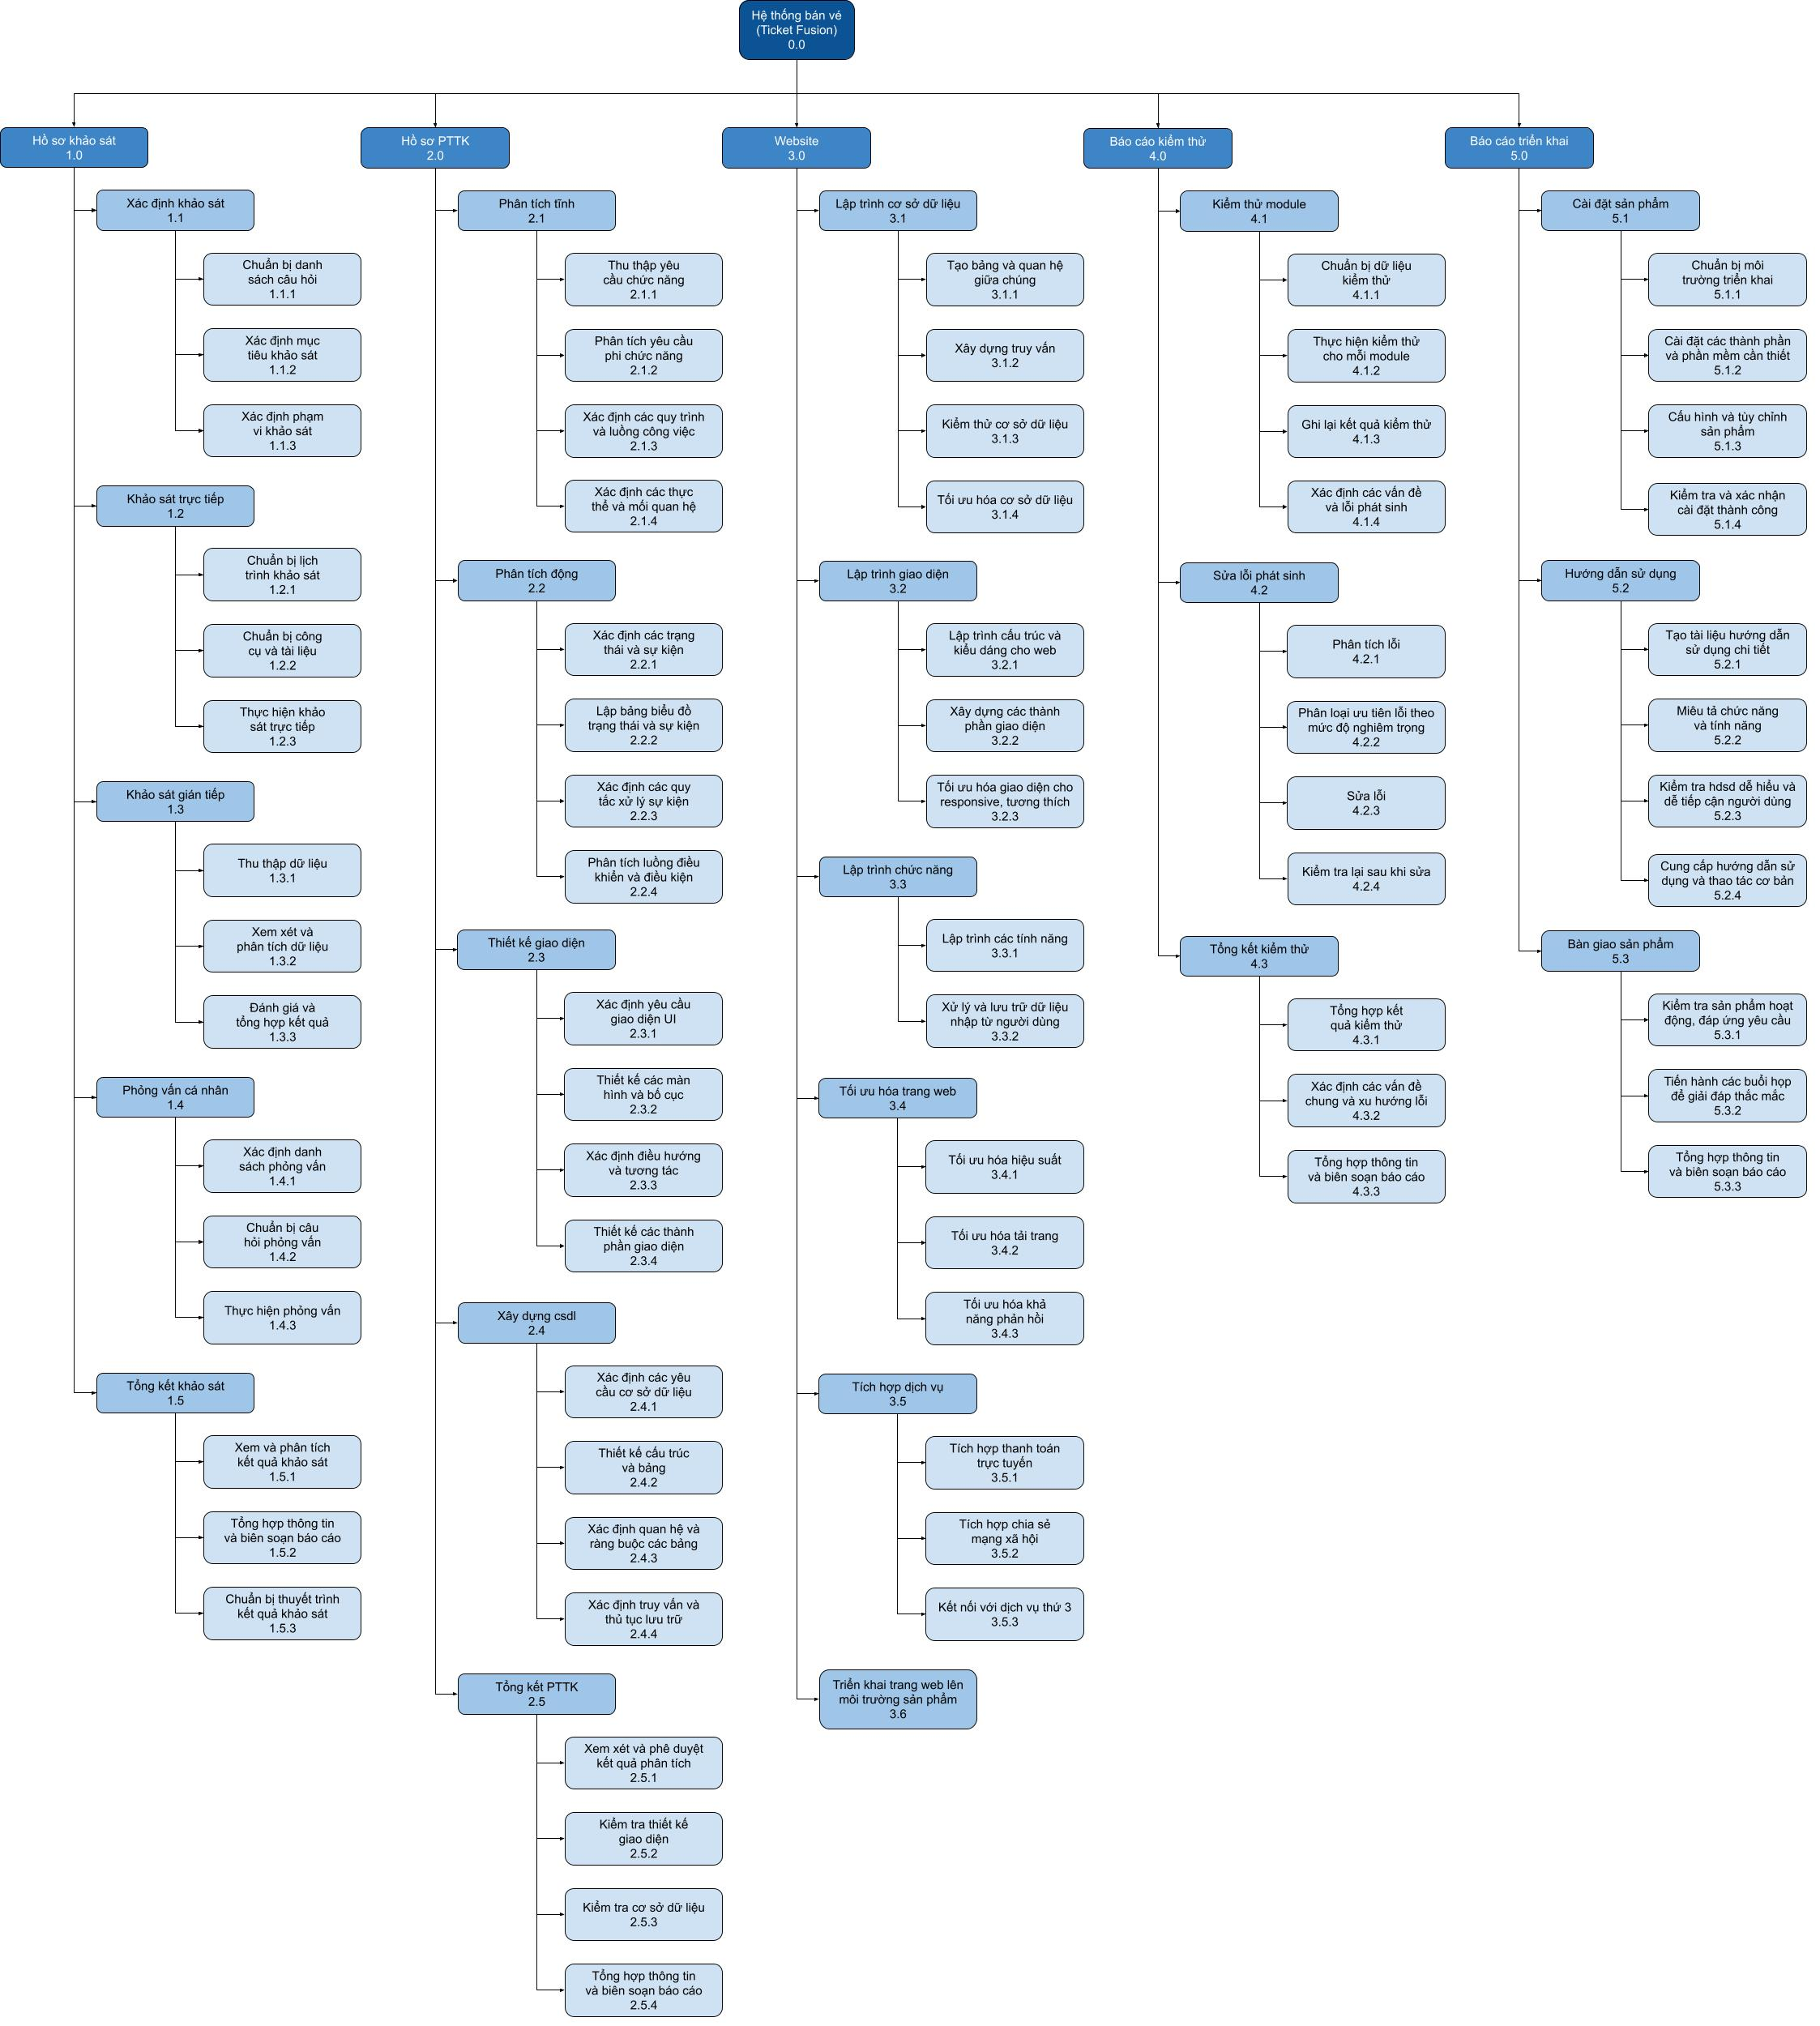
\includegraphics[width=20cm]{WBS.jpg}
\vspace{1cm}
\newpage
\subsection{Quản lý phạm vi}
\subsubsection{Biên bản phạm vi dự án}
\begin{itemize}[label=-, leftmargin=1cm]
    \item Tên công việc: Xây dựng nền tảng bán vé trực tuyến TicketFusion
    \item Ngày bắt đầu : 04/09/2023
    \item Ngày kết thúc: 30/11/2023
    \item Người chịu trách nhiệm: Nguyễn Ngọc Bách
    \item Chi phí : 150.000.000 VND
    \item Các yêu cầu của công việc:
    \begin{itemize}[label=+, leftmargin=1cm]
        \item Tài liệu hướng dẫn, điều hành website TicketFusion.
        \item Website TicketFusion.
    \end{itemize}
    \item Các yêu cầu để đánh giá sự thành công của công việc:
    \begin{itemize}[label=+, leftmargin=1cm]
        \item Website đáp ứng yêu cầu các yêu cầu nghiệp vụ của bên đầu tư.
        \item Sử dụng đúng hạn mức chi phí cho phép là 150 triệu đồng.
        \item Website thân thiện với người dùng, thao tác nhanh chóng, hạn chế tối đa các trường hợp lỗi.
        \item Hoàn thành việc cài đặt hệ thống, hướng dẫn sử dụng và bàn giao hệ thống thành công theo đúng yêu cầu của khách hàng.
    \end{itemize}
\end{itemize}

\subsubsection{Phạm vi công việc Khảo sát và phân tích yêu cầu}
\begin{itemize}[label=-, leftmargin=1cm]
    \item Tên công việc : Khảo sát và phân tích yêu cầu
    \item Ngày bắt đầu : 04/09/2023
    \item Ngày kết thúc: 12/09/2023
    \item Người chịu trách nhiệm: Nguyễn Ngọc Bách
    \item Chi phí : 8.000.000 VND
    \item Lý giải về công việc: Bước đầu của dự án sẽ là gặp gỡ, trao đổi với khách hàng về yêu cầu dự án của họ , phân tích và tổng hợp yêu cầu của khách hàng.
    \item Các yêu cầu của công việc:
    \begin{itemize}[label=+, leftmargin=1cm]
        \item Tài liệu khảo sát yêu cầu.
        \item Tài liệu phân tích yêu cầu.
    \end{itemize}
    \item Các yêu cầu để đánh giá sự thành công của công việc:
    \begin{itemize}[label=+, leftmargin=1cm]
        \item Báo cáo tài liệu phân tích yêu cầu khách hàng rõ ràng, dễ hiểu.
        \item Sử dụng đúng hạn mức chi phí cho phép là 8 triệu đồng.
        \item Hoàn thành công việc trong thời gian quy định.
    \end{itemize}
\end{itemize}

\subsubsection{Phạm vi công việc Phân tích thiết kế}
\begin{itemize}[label=-, leftmargin=1cm]
    \item Tên công việc : Phân tích và thiết kế hệ thống
    \item Ngày bắt đầu : 13/09/2023
    \item Ngày kết thúc: 29/09/2023
    \item Người chịu trách nhiệm: Nguyễn Đức Minh
    \item Chi phí : 20.000.000 VND
    \item Lý giải về công việc: Sau khi có tài liệu báo cáo phân tích và tổng hợp yêu cầu của khách hàng chúng ta bắt đầu đặc tả, thiết kế cơ sở dữ liệu và hệ thống website cần xây dựng.
    \item Các yêu cầu của công việc:
    \begin{itemize}[label=+, leftmargin=1cm]
        \item Tài liệu đặc tả hệ thống.
        \item Tài liệu thiết kế hệ thống.
    \end{itemize}
    \item Các yêu cầu để đánh giá sự thành công của công việc:
    \begin{itemize}[label=+, leftmargin=1cm]
        \item Hoàn thành việc đặc tả và thiết kế hệ thống theo đúng tài liệu phân tích yêu cầu của khách hàng.
        \item Sử dụng đúng hạn mức chi phí cho phép là 20 triệu đồng.
        \item Hoàn thành công việc trong thời gian quy định.
    \end{itemize}
\end{itemize}

\subsubsection{Phạm vi công việc Thiết kế Website}
\begin{itemize}[label=-, leftmargin=1cm]
    \item Tên công việc : Thiết kế Website
    \item Ngày bắt đầu : 02/10/2023
    \item Ngày kết thúc: 30/10/2023
    \item Người chịu trách nhiệm: Nguyễn Đức Anh
    \item Chi phí : 23.000.000 VND
    \item  Lý giải về công việc: Sau khi có tài liệu báo cáo đặc tả và thiết kế hệ thống website cần xây dựng, chúng ta bắt đầu vào thực hiện xây dựng website bằng việc lập trình CSDL, giao diện và chức năng.
    \item Các yêu cầu của công việc:
    \begin{itemize}[label=+, leftmargin=1cm]
        \item Cơ sở dữ liệu.
        \item Giao diện UI/UX.
        \item Code chức năng.
        \item Website.
    \end{itemize}
    \item Các yêu cầu để đánh giá sự thành công của công việc:
    \begin{itemize}[label=+, leftmargin=1cm]
        \item Hoàn thành việc lập trình website theo đúng tài liệu đặc tả và thiết kế hệ thống.
        \item Sử dụng đúng hạn mức chi phí cho phép là 23 triệu đồng.
        \item Hoàn thành công việc trong thời gian quy định.
    \end{itemize}
\end{itemize}

\subsubsection{Phạm vi công việc Kiểm thử}
\begin{itemize}[label=-, leftmargin=1cm]
    \item Tên công việc : Kiểm thử
    \item Ngày bắt đầu : 30/10/2023
    \item Ngày kết thúc: 15/11/2023
    \item Người chịu trách nhiệm: Trương Quốc Bảo
    \item Chi phí : 11.000.000 VND
    \item Lý giải về công việc: Sau khi đã xây dựng xong website chúng ta bắt đầu kiểm thử hệ thống xem hệ thống có sai sót gì về chức năng, giao diện so với tài liệu đặc tả và phân tích yêu cầu không.
    \item Các yêu cầu của công việc:
    \begin{itemize}[label=+, leftmargin=1cm]
        \item Tài liệu báo cáo kiểm thử hệ thống.
    \end{itemize}
    \item Các yêu cầu để đánh giá sự thành công của công việc:
    \begin{itemize}[label=+, leftmargin=1cm]
        \item Hoàn thành việc kiểm thử hệ thống không còn bất kỳ sai sót nào trong quá trình hoạt động hệ thống.
        \item Sử dụng đúng hạn mức chi phí cho phép là 11 triệu đồng.
        \item Hoàn thành công việc trong thời gian quy định.
    \end{itemize}
\end{itemize}

\subsubsection{Phạm vi công việc Triển khai và bàn giao}
\begin{itemize}[label=-, leftmargin=1cm]
    \item Tên công việc : Triển khai và bàn giao
    \item Ngày bắt đầu : 16/11/2023
    \item Ngày kết thúc: 24/11/2023
    \item Người chịu trách nhiệm: Phạm Quỳnh Anh
    \item Chi phí : 11.000.000 VND
    \item Lý giải về công việc: Sau khi đã hoàn thành xây dựng và kiểm thử hệ thống chúng ta sẽ tiến hành cài đặt, hướng dẫn sử dụng, bàn giao hệ thống cho khách hàng.
    \item Các yêu cầu của công việc:
    \begin{itemize}[label=+, leftmargin=1cm]
        \item Tài liệu báo cáo bàn giao dự án.
    \end{itemize}
    \item Các yêu cầu để đánh giá sự thành công của công việc:
    \begin{itemize}[label=+, leftmargin=1cm]
        \item Hoàn thành việc cài đặt hệ thống, hướng dẫn sử dụng và bàn giao hệ thống thành công theo đúng yêu cầu của khách hàng.
        \item Sử dụng đúng hạn mức chi phí cho phép là 11 triệu đồng.
        \item Hoàn thành công việc trong thời gian quy định.
    \end{itemize}
\end{itemize}

\subsection{Quản lý thời gian}
\hspace{1cm}- Dự án quản lý xây dựng Website bán vé sự kiện (Ticket Fusion) do nhà đầu tư Trần Hồng Diệp đầu tư với vốn 150.000.000 đồng yêu cầu hoàn thành dự án trong vòng khoảng 3 tháng từ ngày 04/09/2023 đến ngày 24/11/2023

\subsubsection{Các mốc thời gian quan trọng}
\begin{tabularx}{\linewidth}{|>{\centering\arraybackslash}p{1.7cm}|>{\centering\arraybackslash}p{1.4cm}|>{\centering\arraybackslash}p{1.4cm}|>{\centering\arraybackslash}p{1.4cm}|>{\centering\arraybackslash}p{1.4cm}|>{\centering\arraybackslash}p{1.4cm}|>{\centering\arraybackslash}p{1.4cm}|>{\centering\arraybackslash}p{1.4cm}|}
    \hline
         & \cellcolor[HTML]{C6D9F1}\rule{0pt}{0.6cm}\textbf{\fontsize{6}{9}\selectfont 04/09/2023 - 07/09/2023 \vspace{-0.2cm}} 
         & \cellcolor[HTML]{C6D9F1}\textbf{\fontsize{6}{9}\selectfont 08/09/2023 - 12/09/2023} 
         & \cellcolor[HTML]{C6D9F1}\textbf{\fontsize{6}{9}\selectfont 13/09/2023
         - 27/09/2023} 
         & \cellcolor[HTML]{C6D9F1}\textbf{\fontsize{6}{9}\selectfont 21/09/2023 - 27/09/2023} 
         & \cellcolor[HTML]{C6D9F1}\textbf{\fontsize{6}{9}\selectfont 02/10/2023 - 30/10/2023} 
         & \cellcolor[HTML]{C6D9F1}\textbf{\fontsize{6}{9}\selectfont 30/10/2023 - 15/11/2023}
         & \cellcolor[HTML]{C6D9F1}\textbf{\fontsize{6}{9}\selectfont 16/11/2023 - 24/11/2023}
          \\
    \hline
        \rule{0pt}{0.6cm}{Kết thúc khảo sát \vspace{0.3cm}} & X &&&&&& \\
    \hline
        \rule{0pt}{0.6cm}{Kết thúc phân tích yêu cầu \vspace{0.3cm}} && X &&&&& \\
    \hline
        \rule{0pt}{0.6cm}{Kết thúc phân tích thiết kế \vspace{0.3cm}} &&& X &&&& \\
    \hline
        \rule{0pt}{0.6cm}{Kết thúc xây dựng csdl \vspace{0.3cm}} &&&& X &&& \\
    \hline
        \rule{0pt}{0.6cm}{Kết thúc thiết kế website \vspace{0.3cm}} &&&&& X && \\
    \hline
        \rule{0pt}{0.6cm}{Kết thúc kiểm thử \vspace{0.3cm}} &&&&&& X & \\
    \hline
        \rule{0pt}{0.6cm}{Kết thúc dự án và bàn giao sản phẩm \vspace{0.3cm}} &&&&&&& X \\
    \hline
\end{tabularx}

\subsubsection{Ước lượng thời gian}
\begin{itemize}[label=-, leftmargin=1cm]
    \item Được tính dựa trên 3 giá trị thời gian ước lượng với công thức:
        \begin{center}
            \textbf{ET = (MO + 4ML + MP)/6.}
        \end{center}
    \item Ước lượng khả dĩ nhất (ML – Most likely): Thời gian cần để hoàn thành công việc trong điều kiện bình thường hay hợp lý.
    \item Ước lượng lạc quan nhất (MO – Most Optimistic): Thời gian cần để hoàn thành công việc trong điều kiện “tốt nhất” hay “lý tưởng” (không có trở ngại nào).
    \item Ước lượng bi quan nhất (MP - Most Pessimistic): Thời gian cần để hoàn thành công việc một cách “tồi nhất” (nhiều trở ngại).
    \item Thời gian lãng phí cho mỗi công việc thông thường từ (7\% -10\%)
        \begin{center}
            \textbf{ET cuối cùng = ET + ET*8\%}
        \end{center}
    \item Đơn vị tính: Ngày
\end{itemize}
\begin{center}
    \textbf{Giai đoạn 1: Khảo sát và phân tích yêu cầu}
\end{center}
 
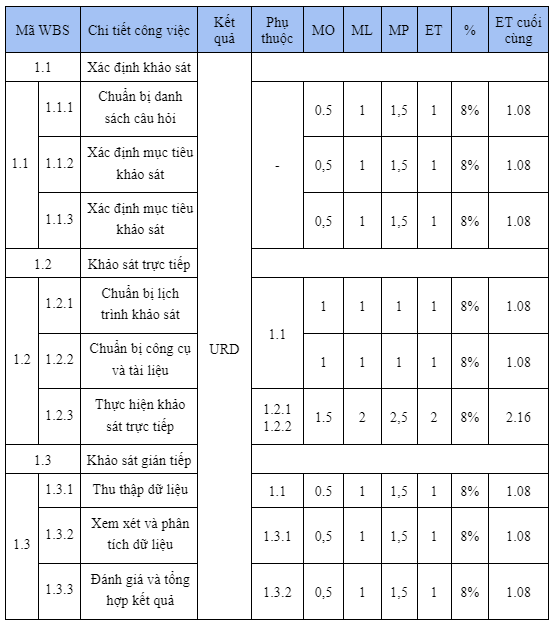
\includegraphics[width=14.5cm]{ThoiGian1_1.png}
\par
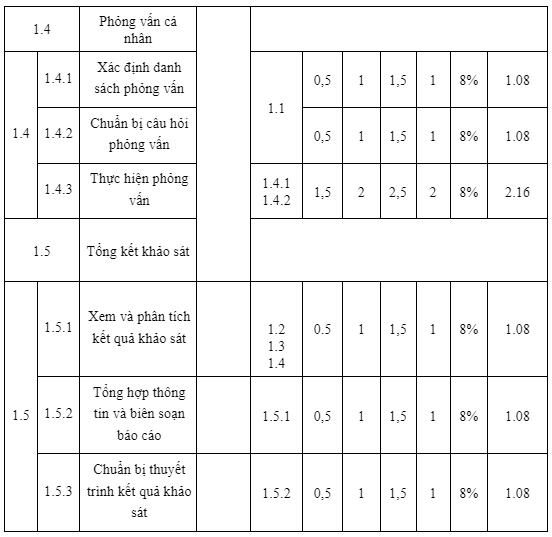
\includegraphics[width=14.5cm]{ThoiGian1_2.png}
\vspace{0.5cm}

\hspace{1cm}\textbf{- PERT-AON Thời gian hoàn thành sớm nhất \\\\} 
\vspace*{0.5cm}    
\hspace{0.7cm}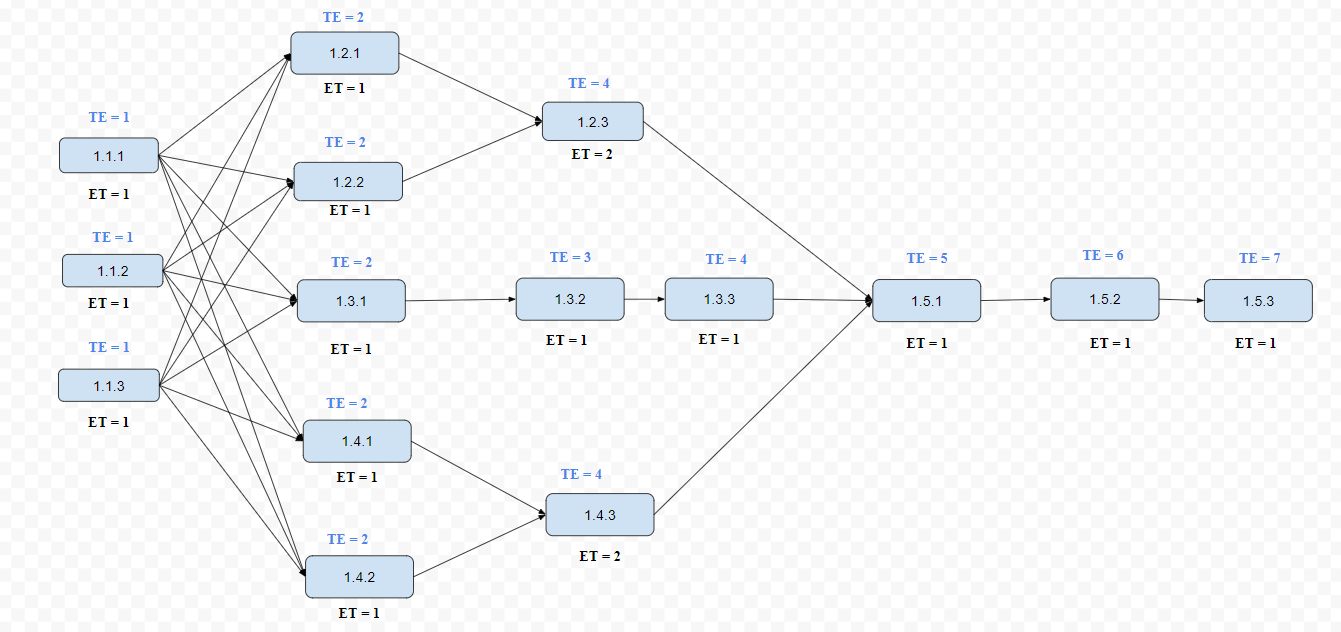
\includegraphics[width=14.5cm]{PERT1_1.png}
\vspace{0.5cm}  

\hspace{1cm}\textbf{- PERT-AON Thời gian hoàn thành trễ nhất \\\\} 
\vspace*{0.5cm}    
\hspace{0.7cm}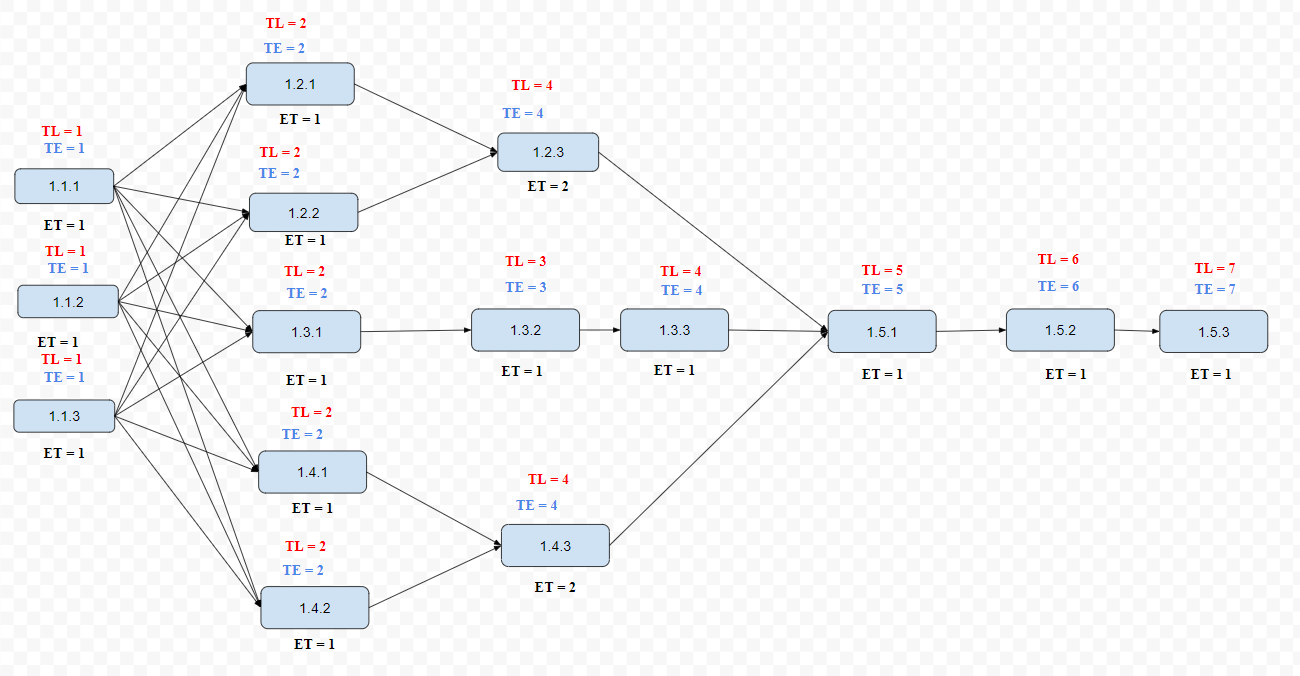
\includegraphics[width=14.5cm]{PERT1_2.png}
\vspace{0.5cm}  

\begin{center}
    \textbf{Giai đoạn 2: Phân tích và thiết kế hệ thống}
\end{center}
 
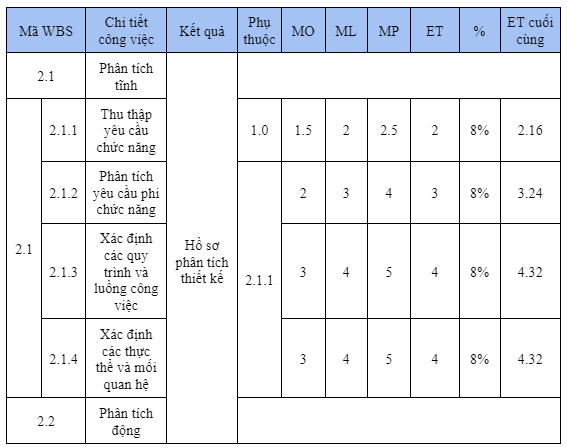
\includegraphics[width=14.5cm]{ThoiGian2_1.png}
\par
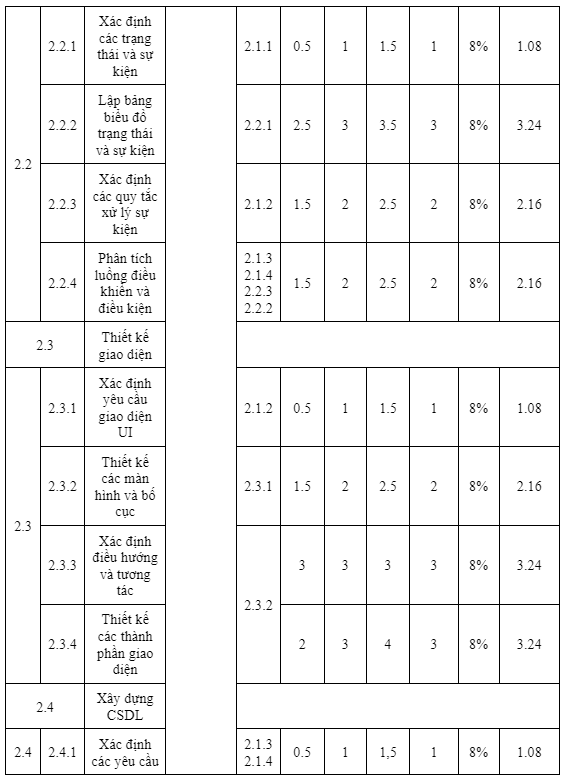
\includegraphics[width=14.5cm]{ThoiGian2_2.png}
\par
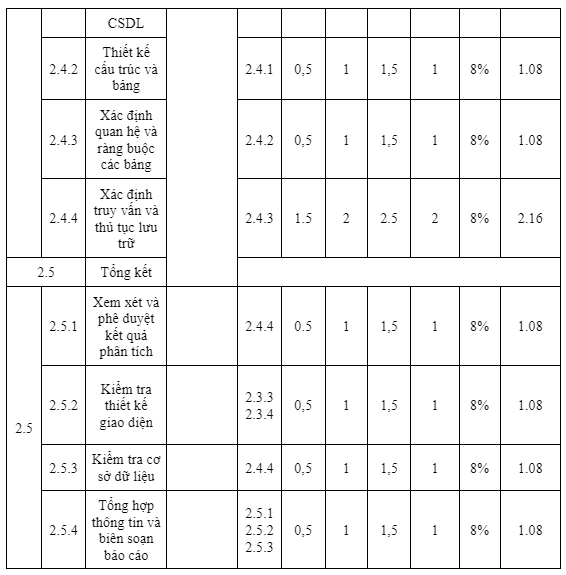
\includegraphics[width=14.5cm]{ThoiGian2_3.png}
\vspace{0.5cm}

\hspace{1cm}\textbf{- PERT-AON Thời gian hoàn thành sớm nhất \\\\} 
\vspace*{0.5cm}    
\hspace{0.7cm}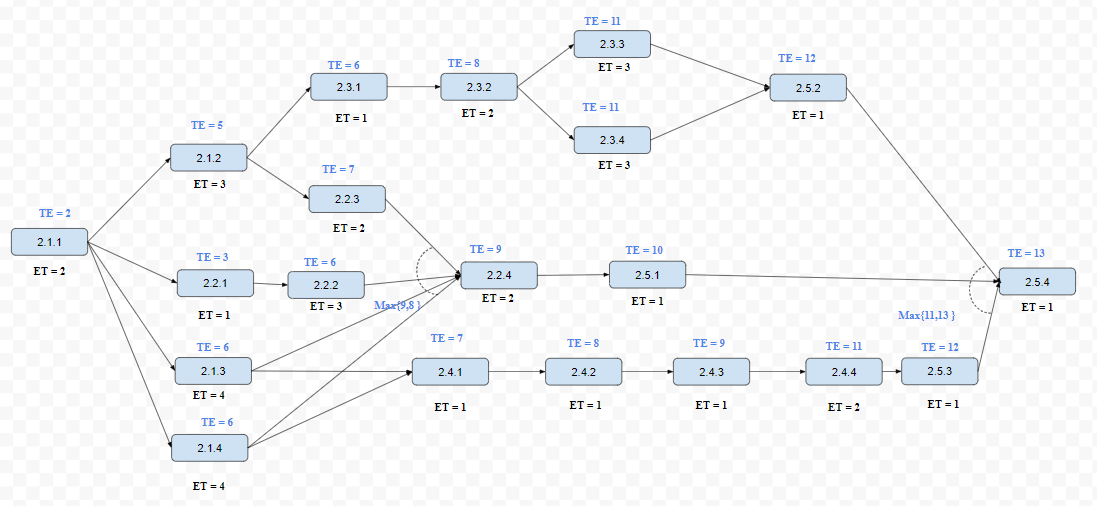
\includegraphics[width=14.5cm]{PERT2_1.png}
\vspace{0.5cm}  

\hspace{1cm}\textbf{- PERT-AON Thời gian hoàn thành trễ nhất \\\\} 
\vspace*{0.5cm}    
\hspace{0.7cm}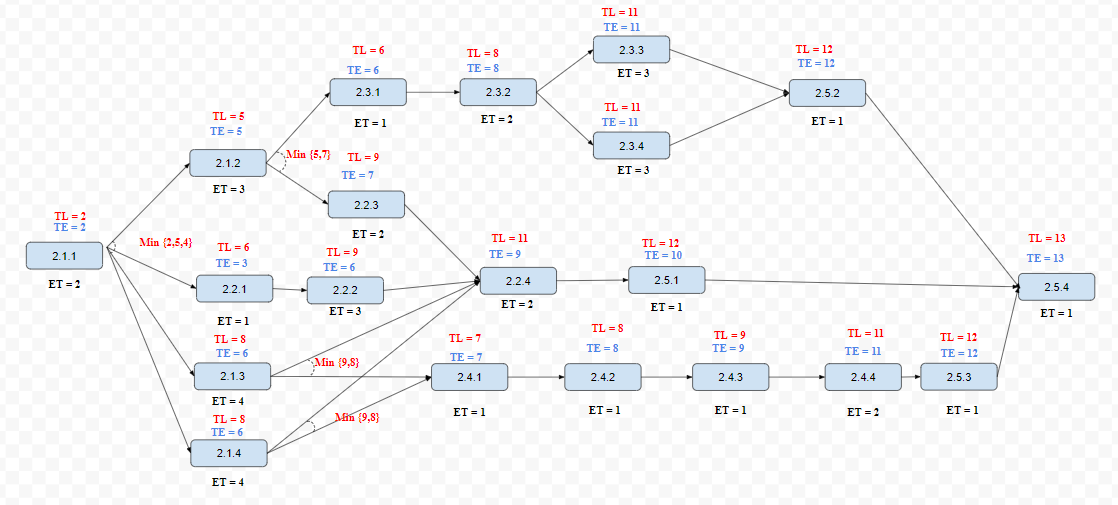
\includegraphics[width=14.5cm]{PERT2_2.png}
\vspace{0.5cm}  

\begin{center}
    \textbf{Giai đoạn 3: Thực hiện}
\end{center}
 
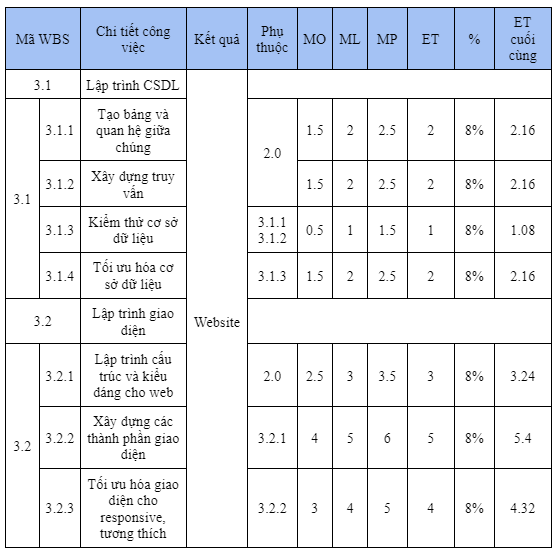
\includegraphics[width=14.5cm]{ThoiGian3_1.png}
\par
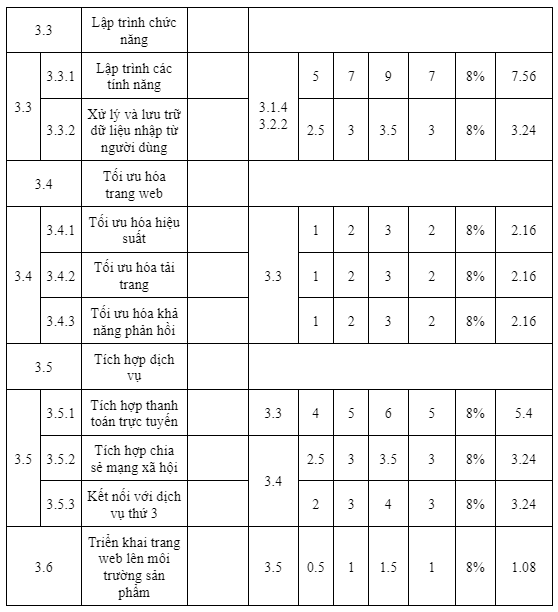
\includegraphics[width=14.5cm]{ThoiGian3_2.png}
\vspace{0.5cm}

\hspace{1cm}\textbf{- PERT-AON Thời gian hoàn thành sớm nhất \\\\} 
\vspace*{0.5cm}    
\hspace{0.7cm}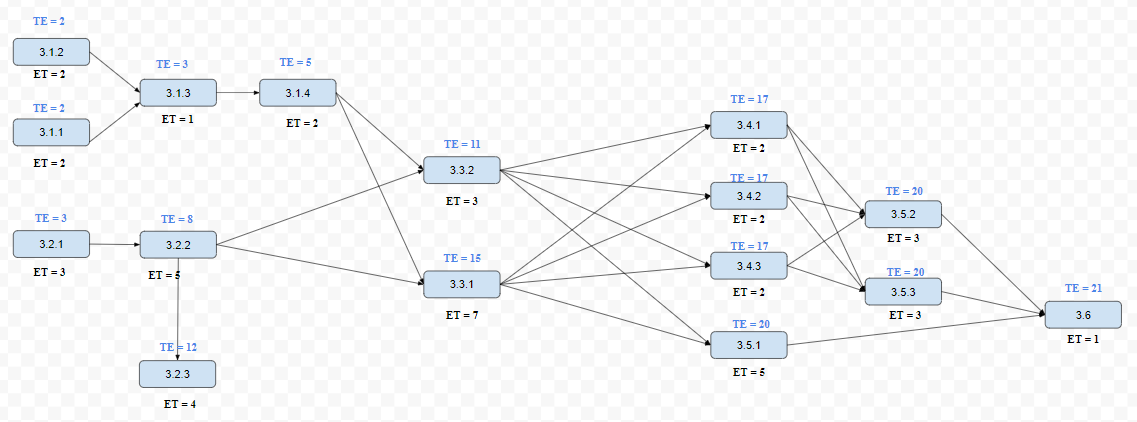
\includegraphics[width=14.5cm]{PERT3_1.png}
\vspace{0.5cm}  

\hspace{1cm}\textbf{- PERT-AON Thời gian hoàn thành trễ nhất \\\\} 
\vspace*{0.5cm}    
\hspace{0.7cm}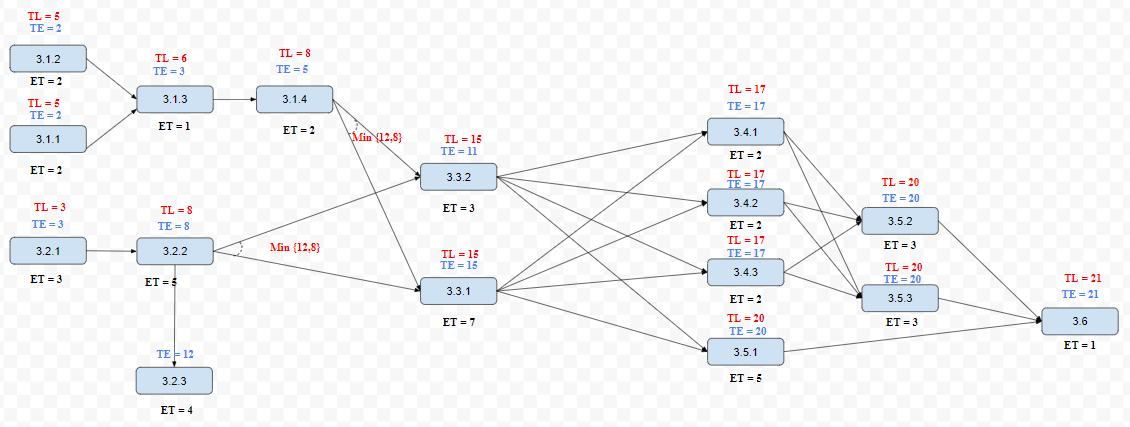
\includegraphics[width=14.5cm]{PERT3_2.png}
\vspace{0.5cm}  

\begin{center}
    \textbf{Giai đoạn 4: Kiểm thử}
\end{center}
 
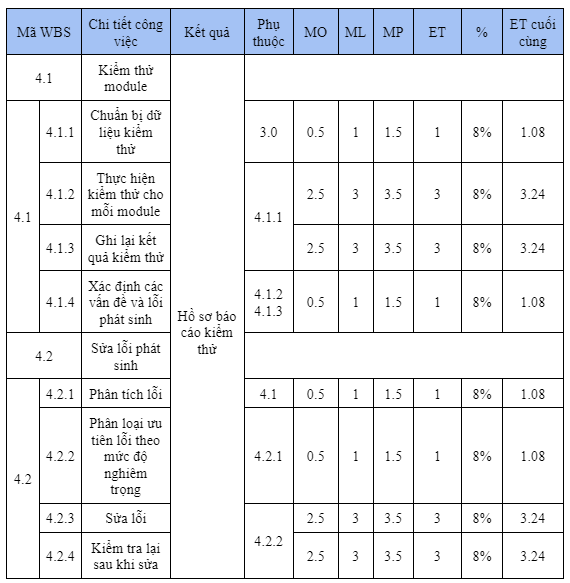
\includegraphics[width=14.5cm]{ThoiGian4_1.png}
\par
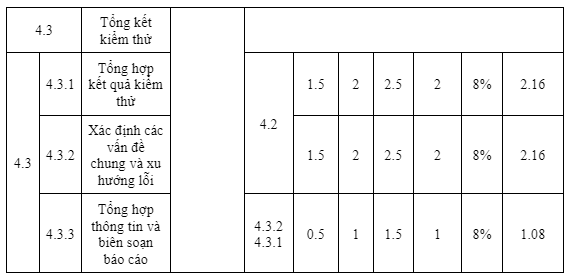
\includegraphics[width=14.5cm]{ThoiGian4_2.png}
\vspace{0.5cm}

\hspace{1cm}\textbf{- PERT-AON Thời gian hoàn thành sớm nhất \\\\} 
\vspace*{0.5cm}    
\hspace{0.7cm}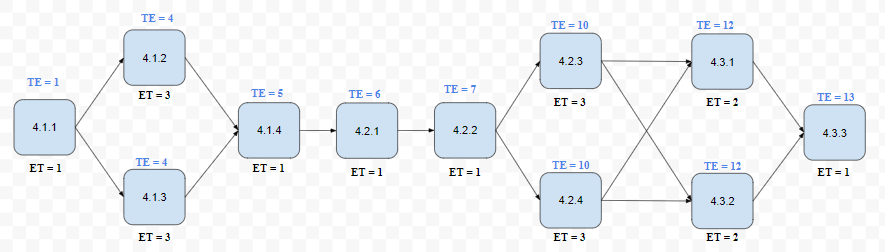
\includegraphics[width=14.5cm]{PERT4_1.png}
\vspace{0.5cm}  

\hspace{1cm}\textbf{- PERT-AON Thời gian hoàn thành trễ nhất \\\\} 
\vspace*{0.5cm}    
\hspace{0.7cm}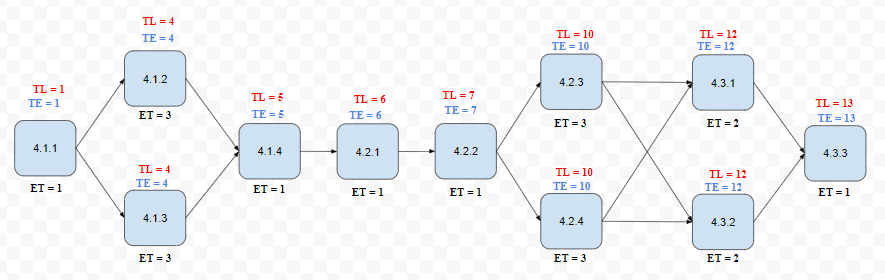
\includegraphics[width=14.5cm]{PERT4_2.png}
\vspace{0.5cm}  

\newpage

\begin{center}
    \textbf{Giai đoạn 5: Triển khai và bàn giao}
\end{center}
 
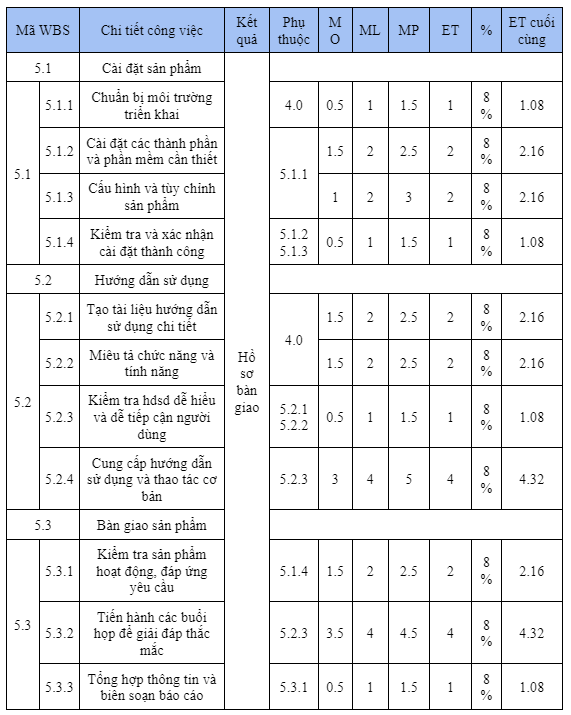
\includegraphics[width=14.5cm]{ThoiGian5_1.png}
\vspace{0.5cm}

\newpage

\hspace{1cm}\textbf{- PERT-AON Thời gian hoàn thành sớm nhất \\\\} 
\vspace*{0.5cm}    
\hspace{0.7cm}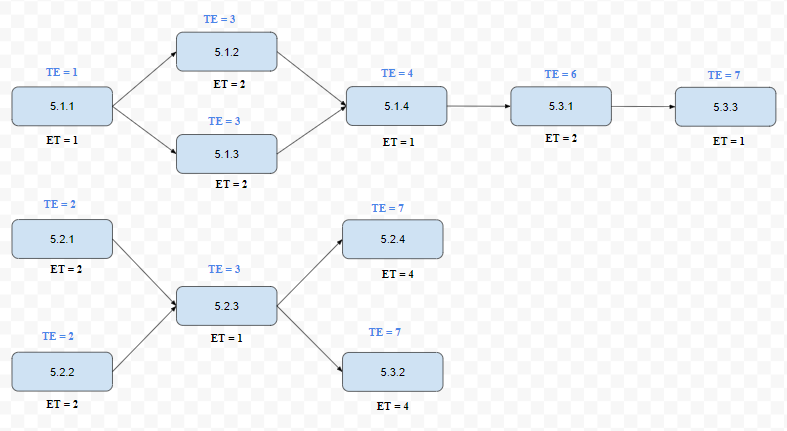
\includegraphics[width=14.5cm]{PERT5_1.png}
\vspace{0.5cm}  

\hspace{1cm}\textbf{- PERT-AON Thời gian hoàn thành trễ nhất \\\\} 
\vspace*{0.5cm}    
\hspace{0.7cm}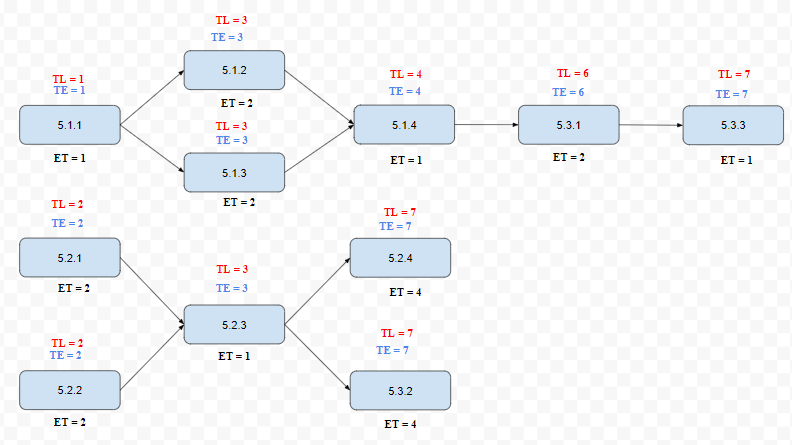
\includegraphics[width=14.5cm]{PERT5_2.png}
\vspace{0.5cm} 

\begin{center}
    \textbf{Bảng ước lượng PERT tổng hợp}
\end{center} 

\hspace{-2cm}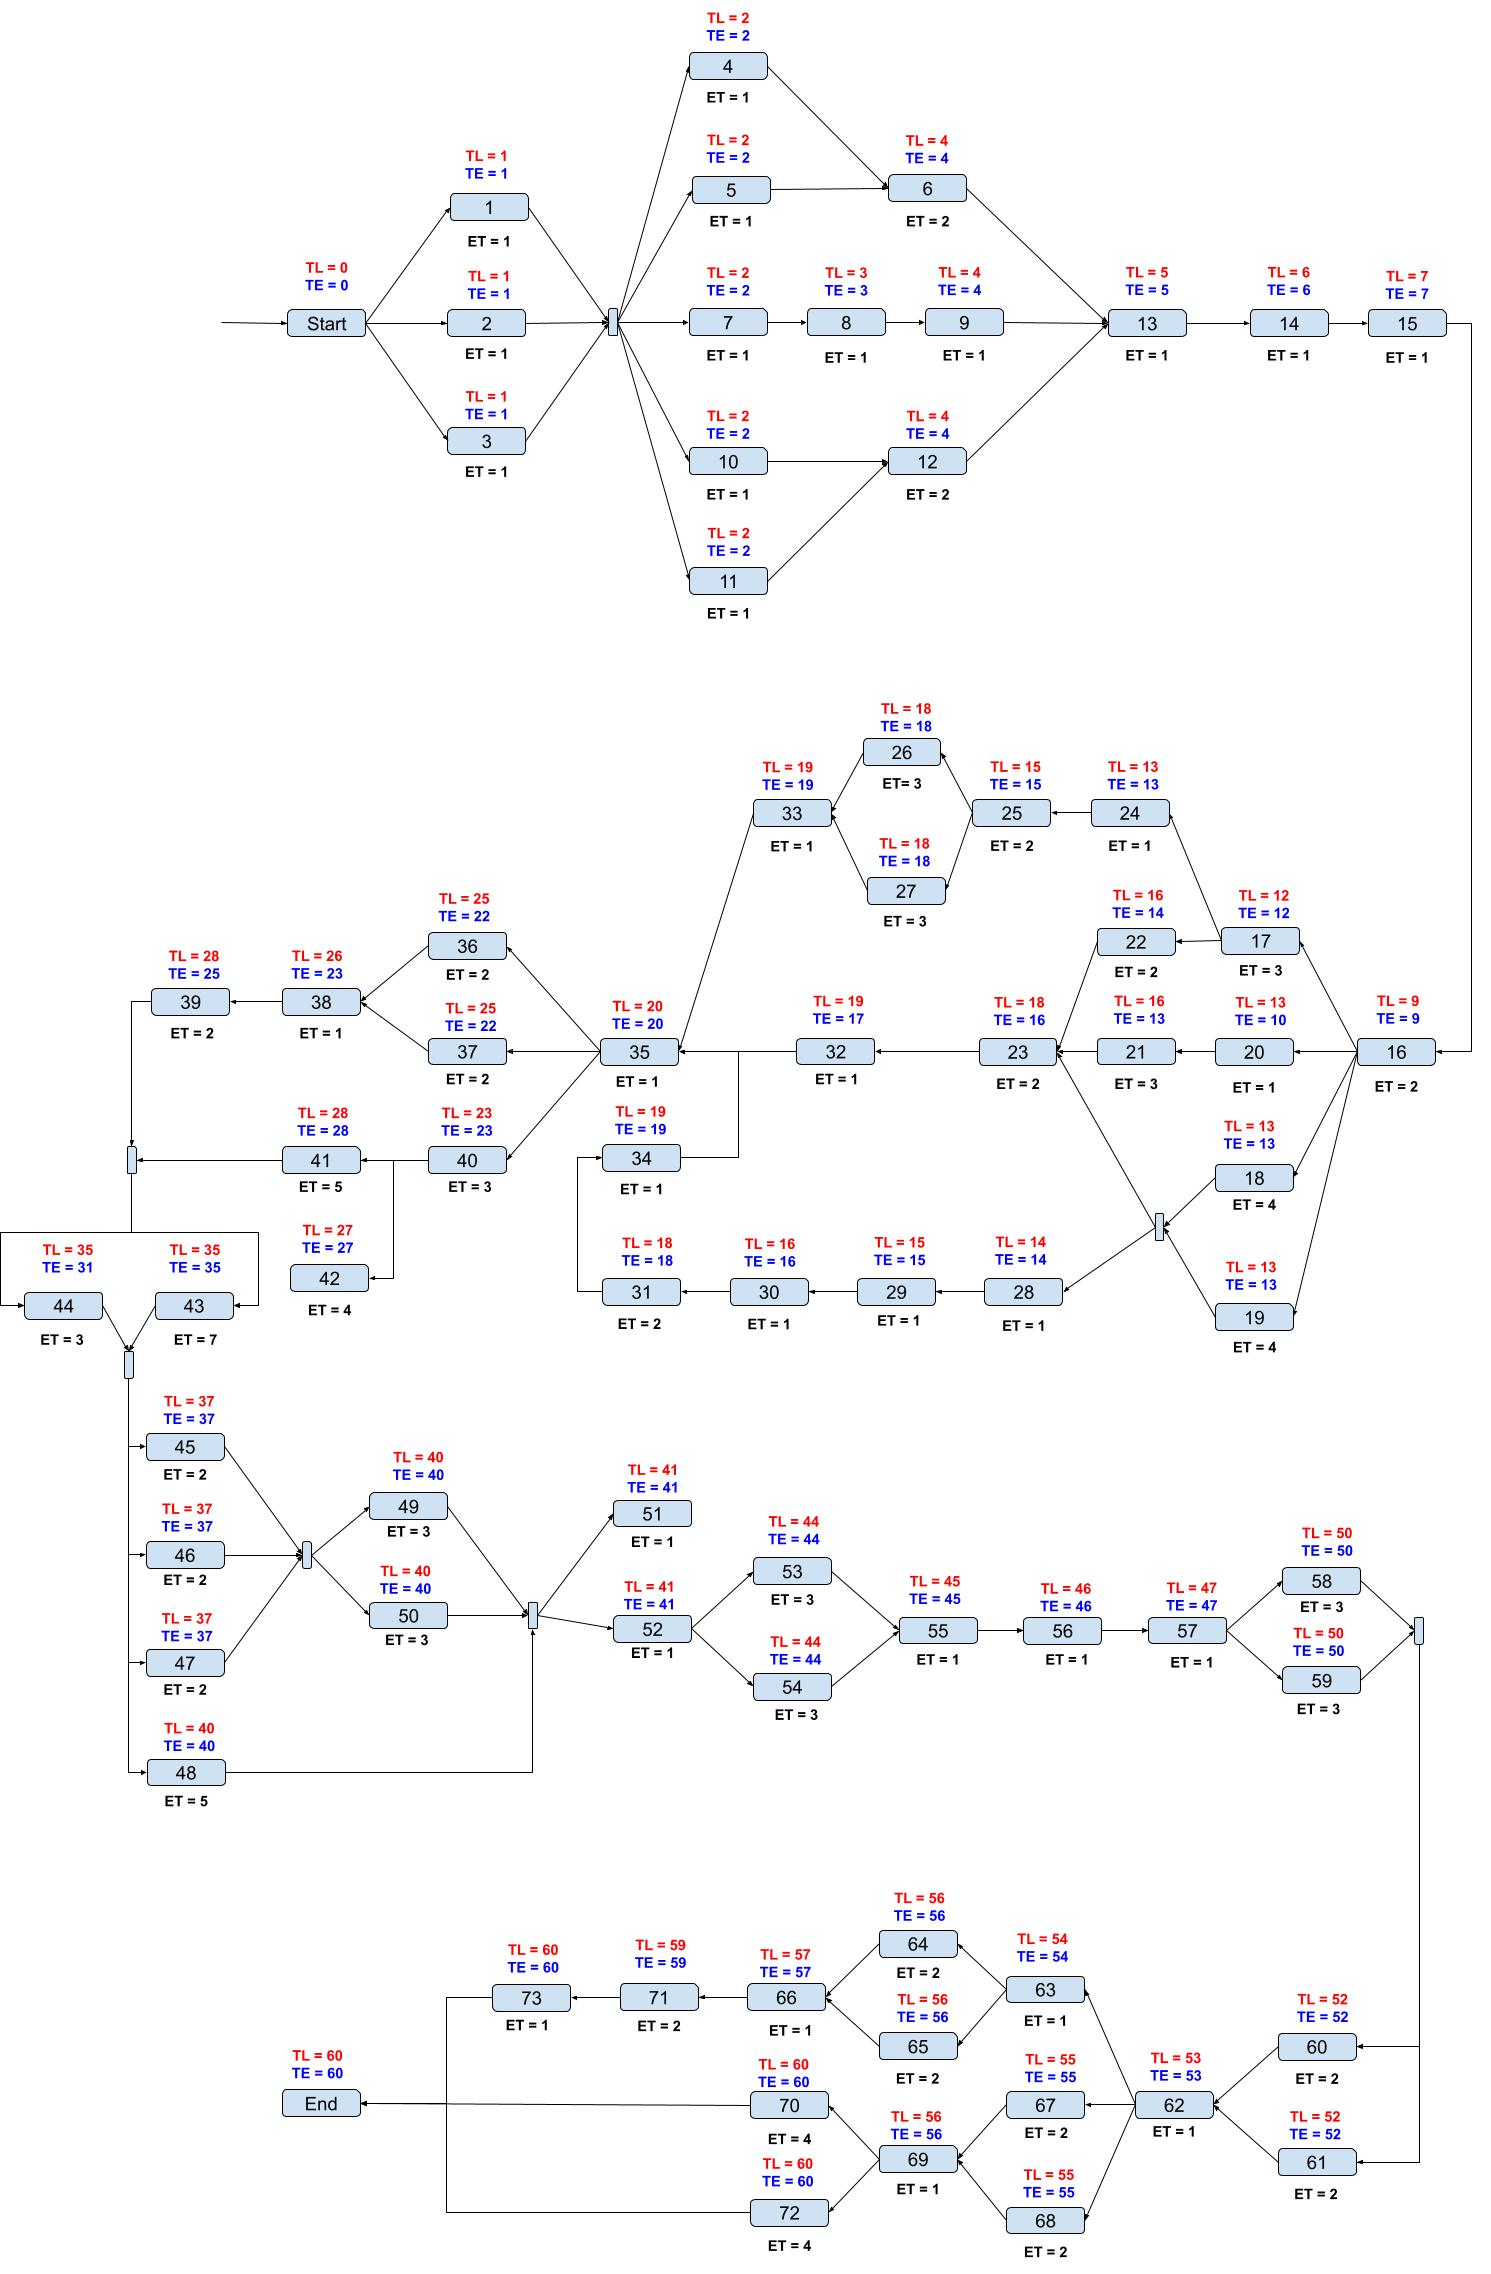
\includegraphics[width=17cm]{PERT2.jpg}
\par
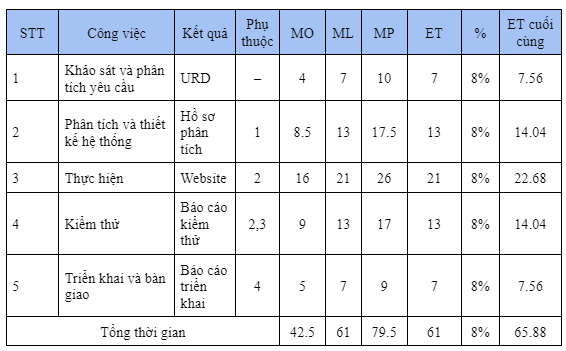
\includegraphics[width=14.5cm]{PERT.png}
\vspace{0.5cm} 

\hspace{1cm}\textbf{- PERT-Action On ARC (AOA) \\\\} 
\vspace*{0.5cm}    
\hspace{0.7cm}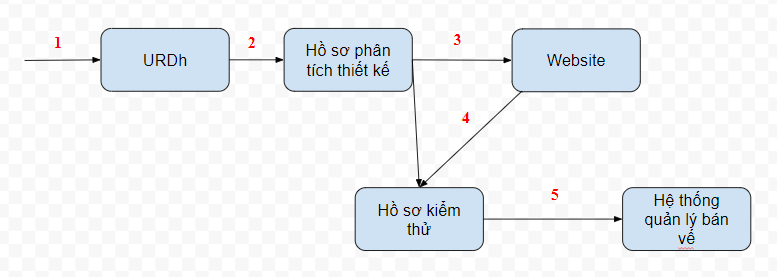
\includegraphics[width=14.5cm]{PERT3.png}
\vspace{0.5cm} 

\hspace{1cm}\textbf{- PERT-Action On Node (AON) \\\\} 
\vspace*{0.5cm}    
\hspace{0.7cm}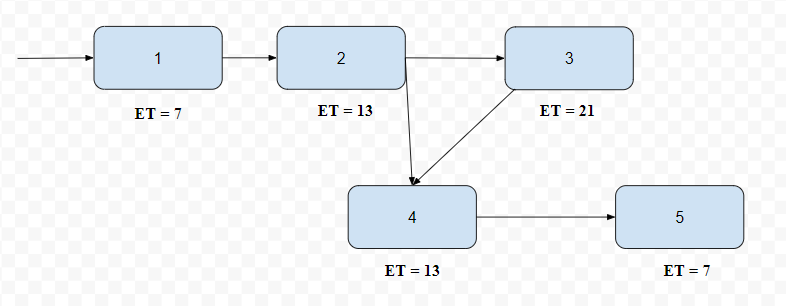
\includegraphics[width=14.5cm]{PERT4.png}
\vspace{0.5cm} 

\hspace{1cm}\textbf{- PERT-AON Thời gian hoàn thành sớm nhất \\\\} 
\vspace*{0.5cm}    
\hspace{0.7cm}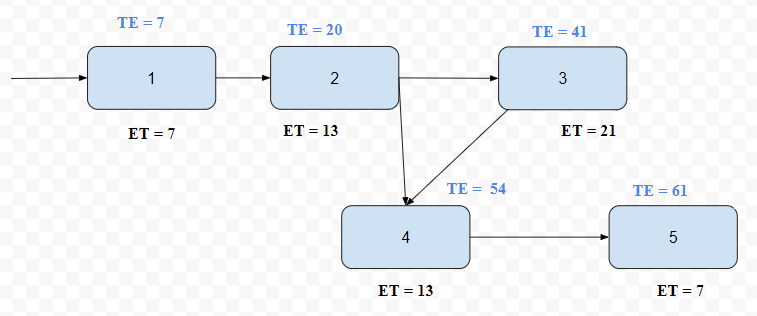
\includegraphics[width=14.5cm]{PERT5.png}
\vspace{0.5cm} 

\hspace{1cm}\textbf{- PERT-AON Thời gian hoàn thành trễ nhất \\\\} 
\vspace*{0.5cm}    
\hspace{0.7cm}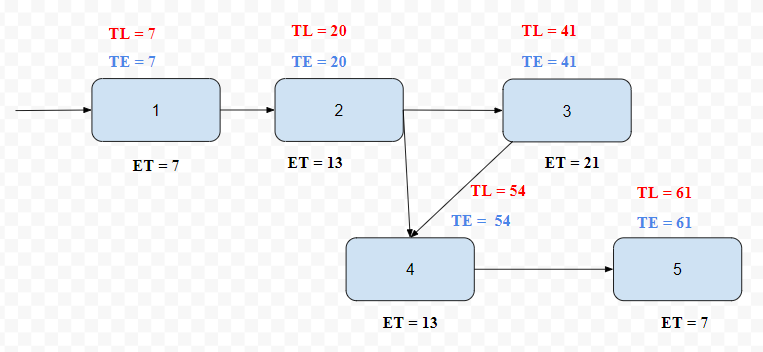
\includegraphics[width=14.5cm]{PERT6.png}
\vspace{0.5cm} 

\subsubsection{Biểu đồ gantt}
\newpage
\hspace{-2.5cm}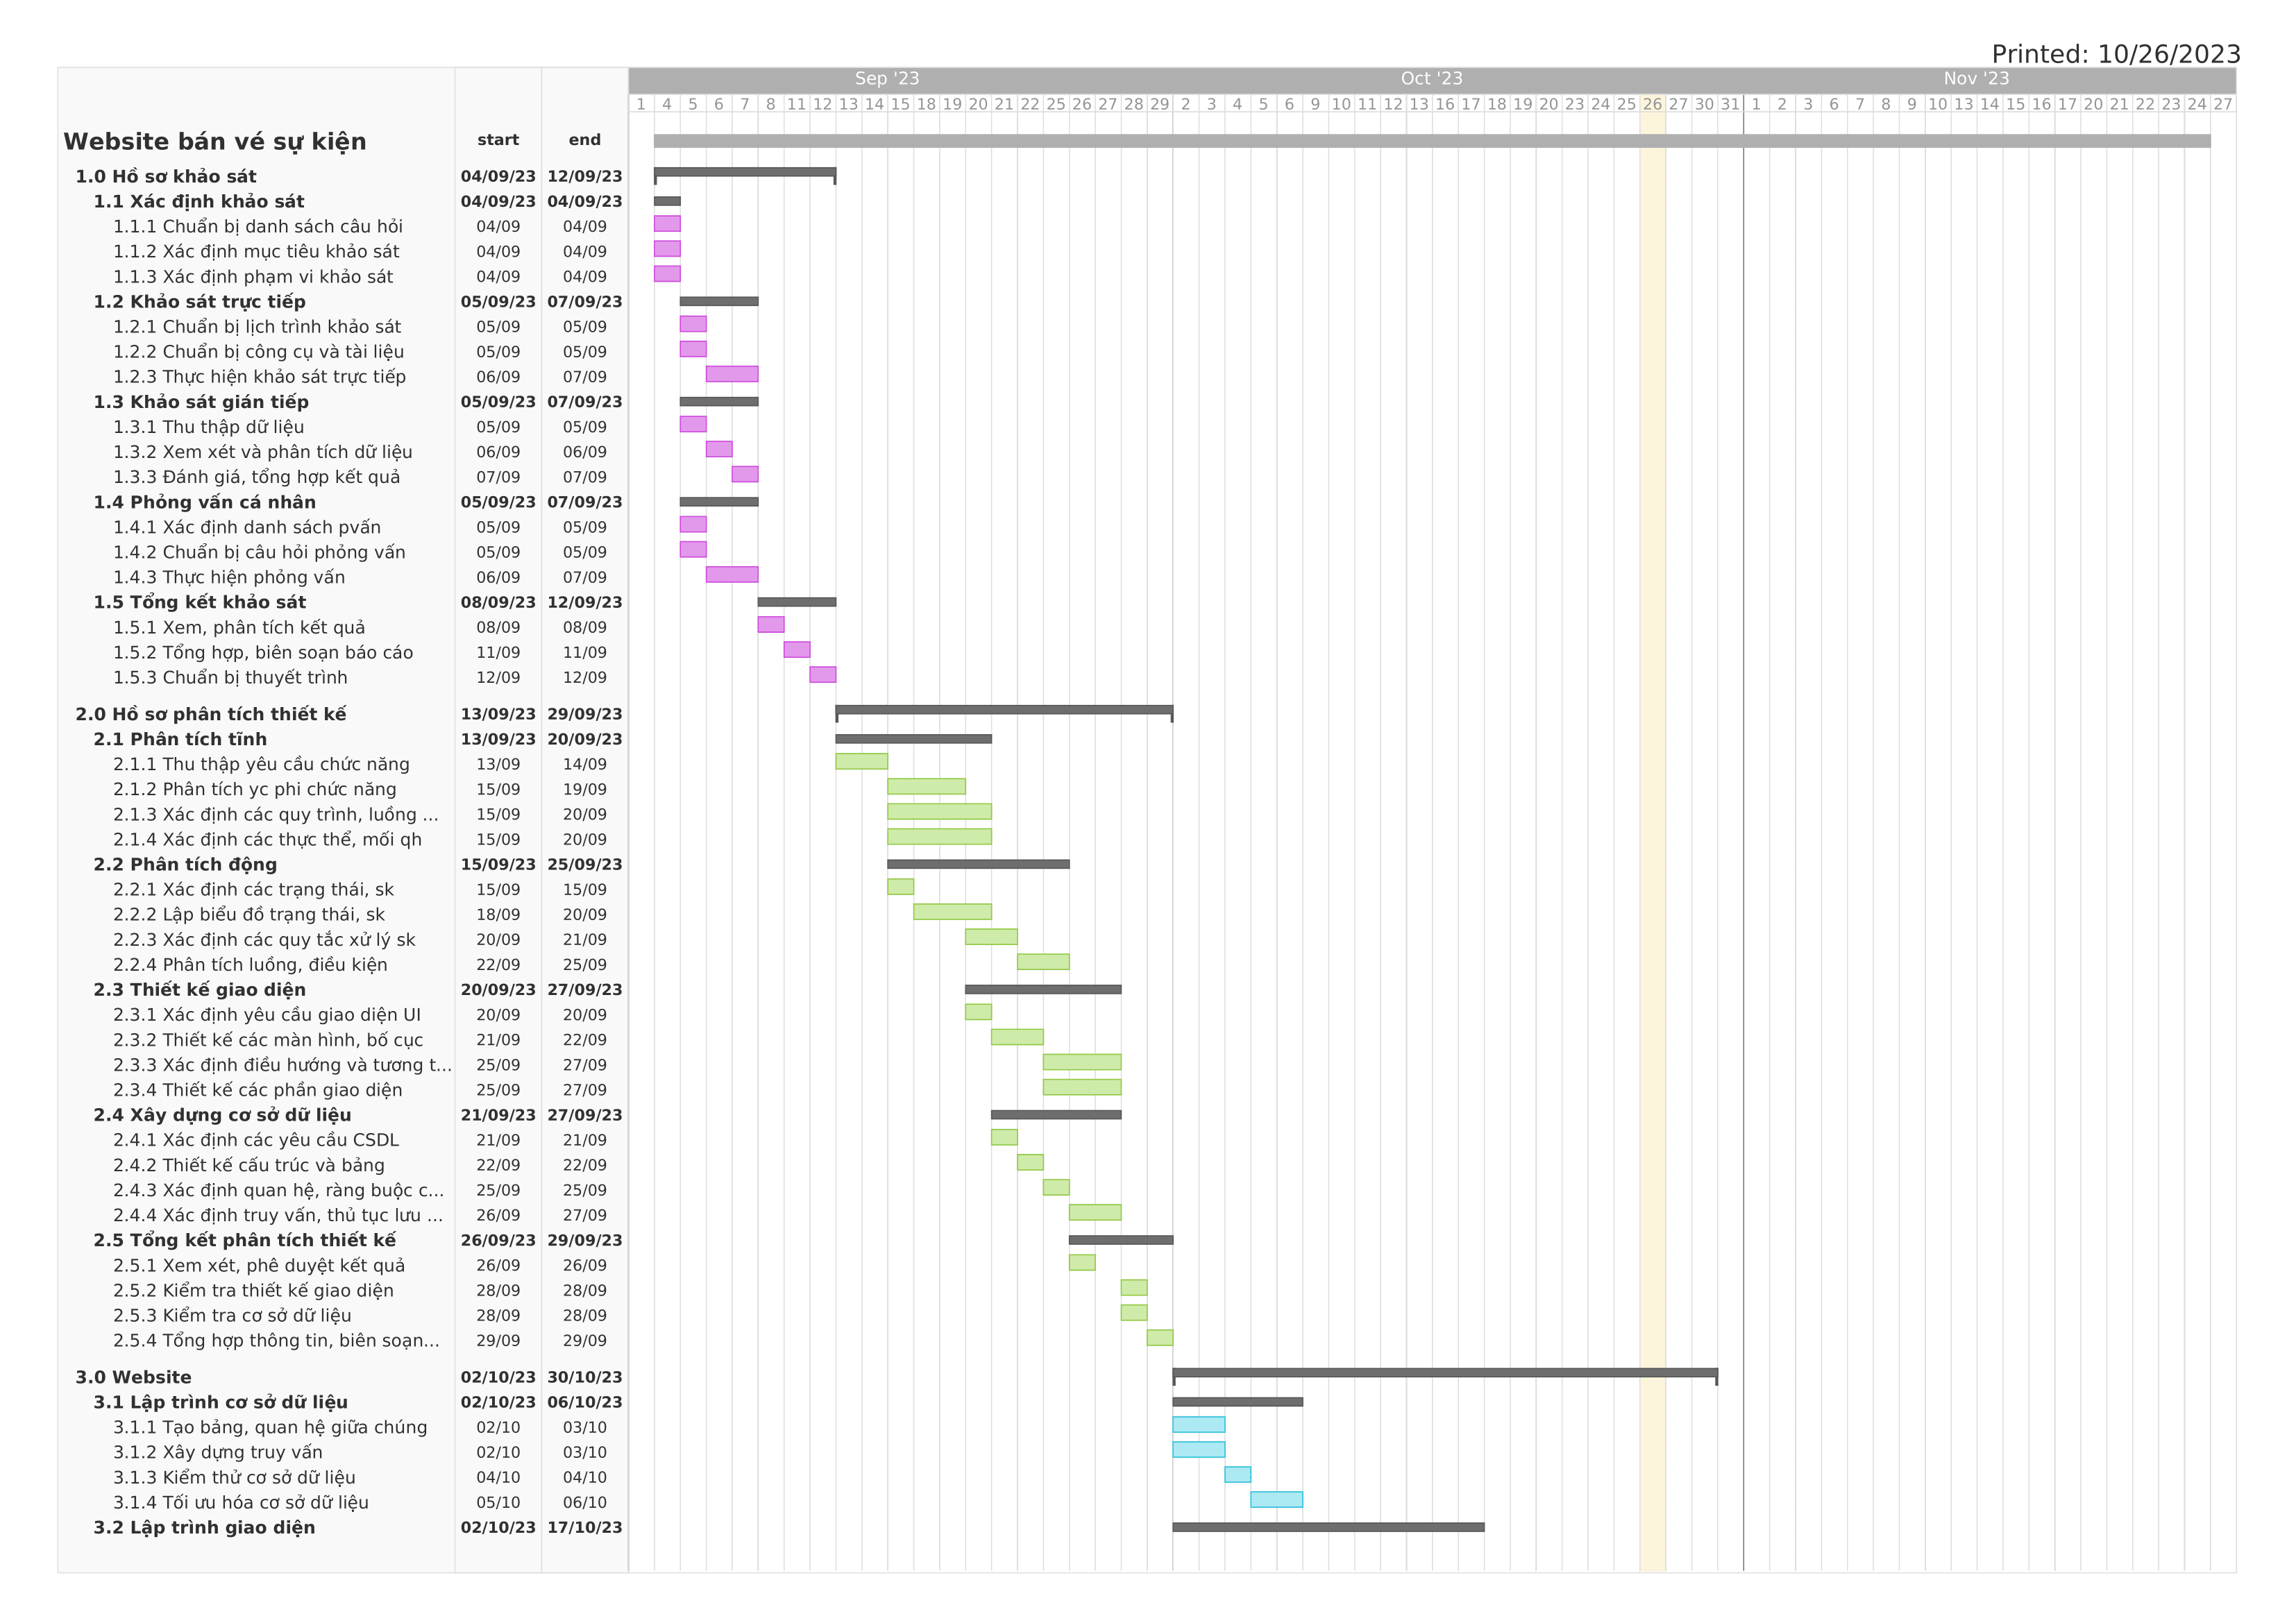
\includegraphics[width=18.5cm]{Gantt_1.png}
\par
\vspace{-0.5cm}
\hspace{-2.5cm}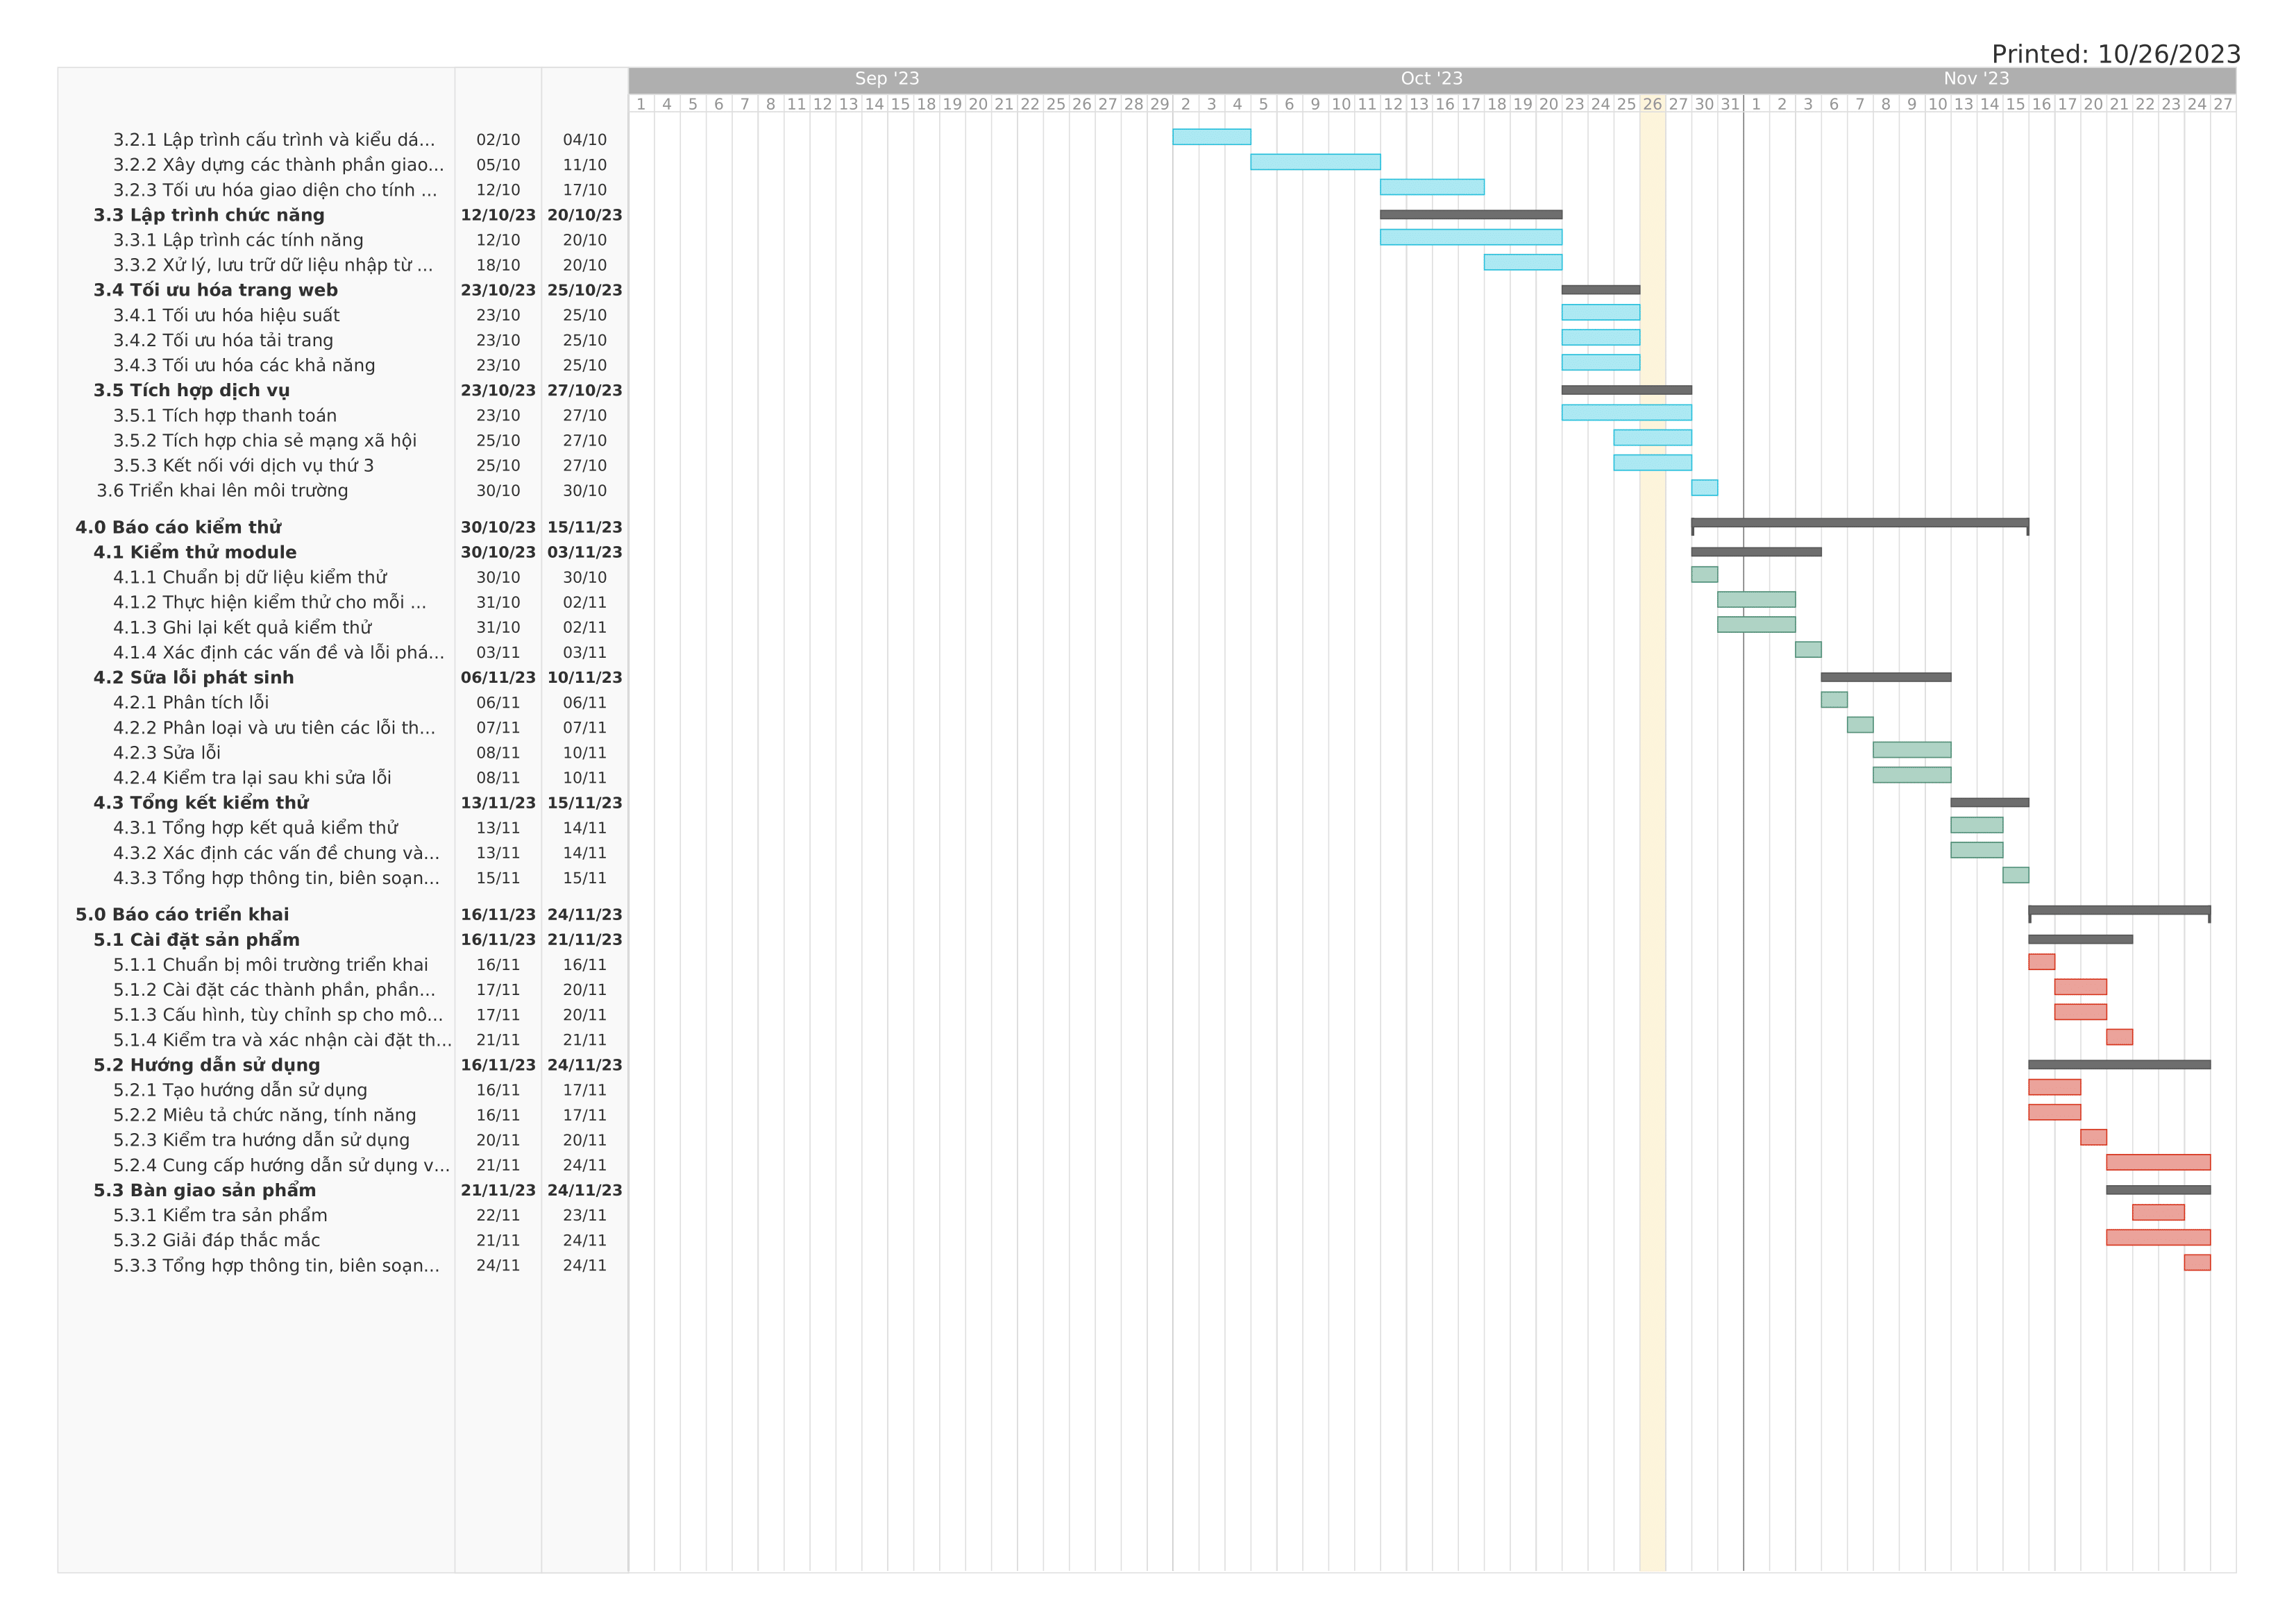
\includegraphics[width=18.5cm]{Gantt_2.png}

=> Như vậy, tổng thời gian công việc hoàn thành theo PERT là ~ 65 ngày, tăng so với thời gian dự kiến cho trước là 5 ngày.

\subsection{Quản lý chi phí}
\subsubsection{Chi phí lương nhân viên}
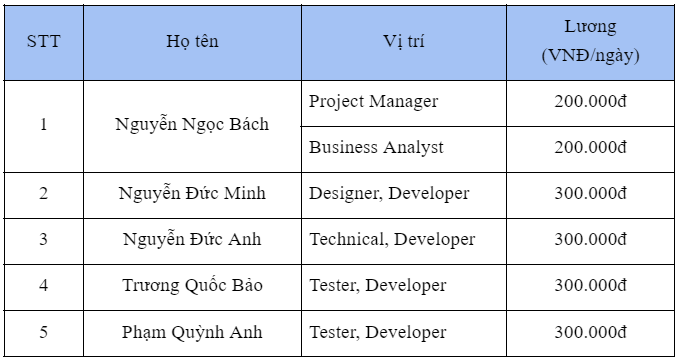
\includegraphics[width=15cm]{Luong0.png}
\vspace{0.5cm}

\subsubsection{Khảo sát và phân tích yêu cầu}
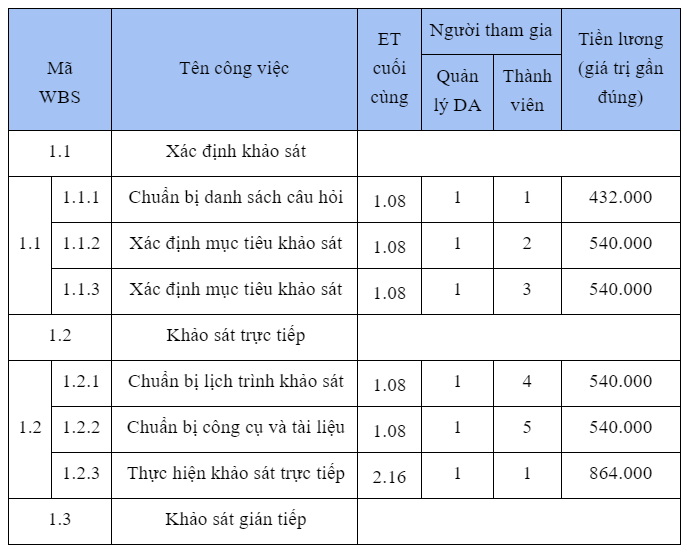
\includegraphics[width=15cm]{ChiPhi1.png}
\par
\hspace{-0.5cm}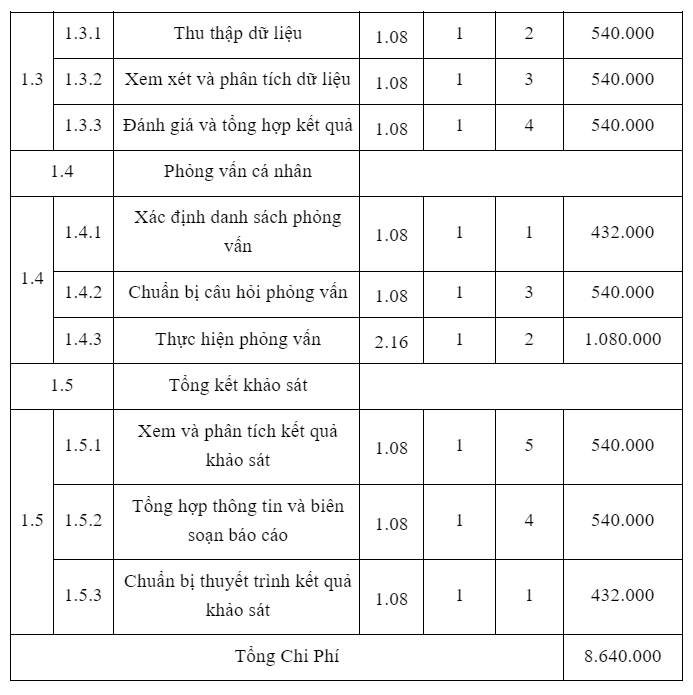
\includegraphics[width=15cm, height=14cm]{ChiPhi2.png}

\subsubsection{Phân tích thiết kế}
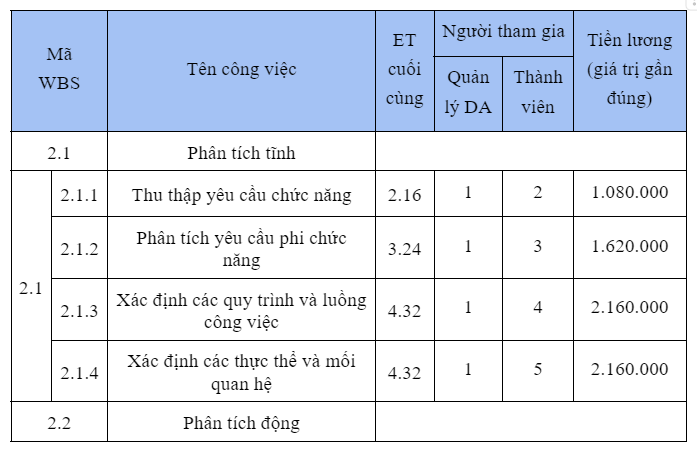
\includegraphics[width=15cm]{ChiPhi3.png}
\par
\hspace{-0.5cm}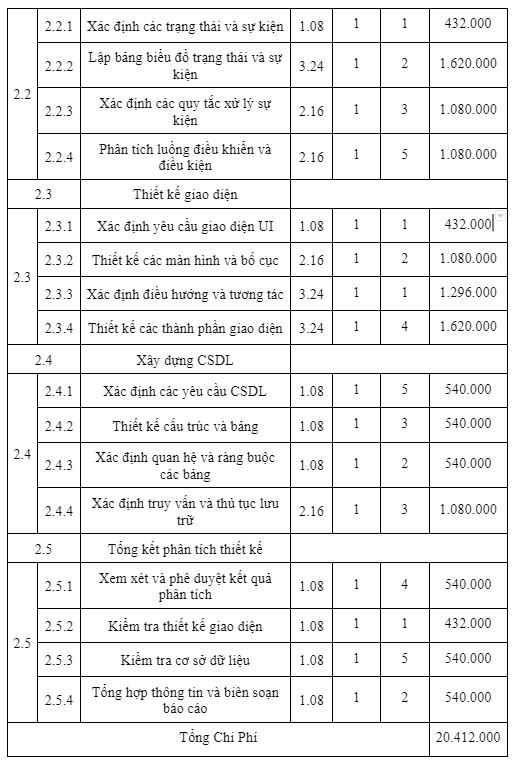
\includegraphics[width=14.5cm]{ChiPhi4.png}
\vspace{0.5cm}

\subsubsection{Thực hiện}
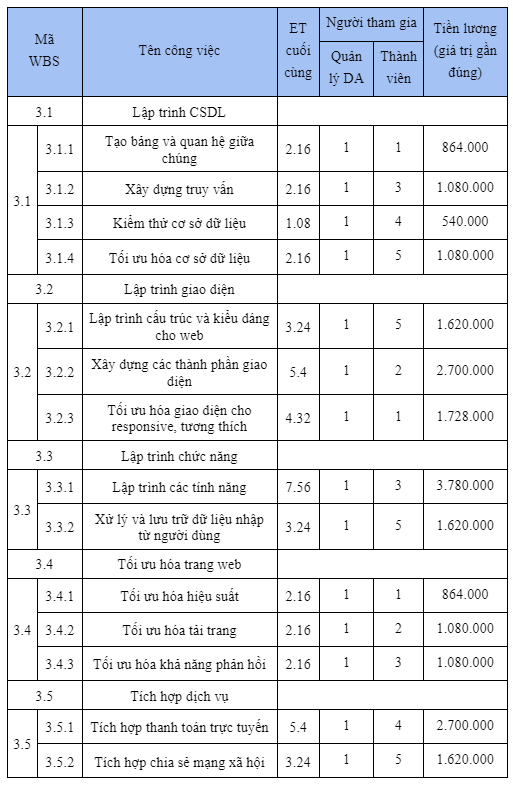
\includegraphics[width=15cm]{ChiPhi5.png}
\par
\hspace{-0.5cm}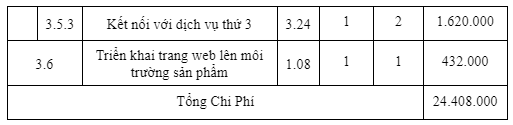
\includegraphics[width=14.5cm]{ChiPhi6.png}
\vspace{0.5cm}

\subsubsection{Kiểm thử}
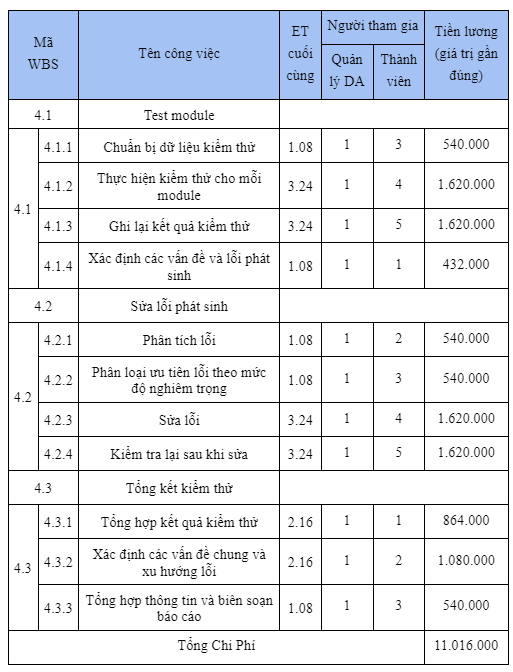
\includegraphics[width=15cm]{ChiPhi7.png}
\vspace{0.5cm}

\subsubsection{Triển khai và bàn giao}
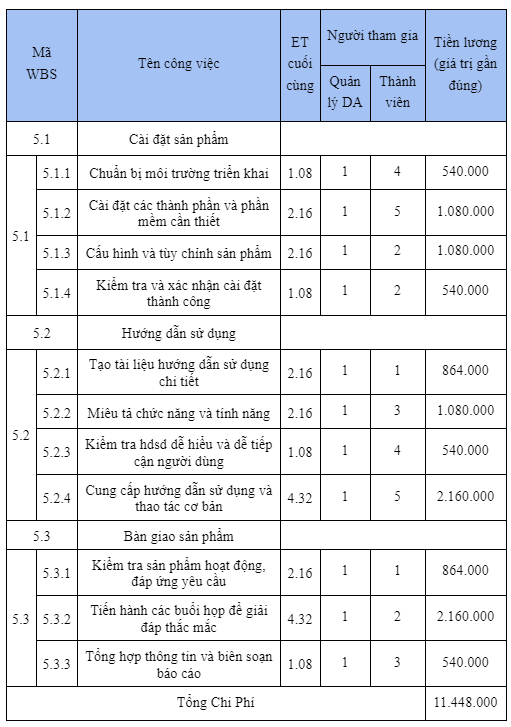
\includegraphics[width=15cm]{ChiPhi8.png}
\vspace{0.5cm}

\subsubsection{Tổng chi phí cho công việc}
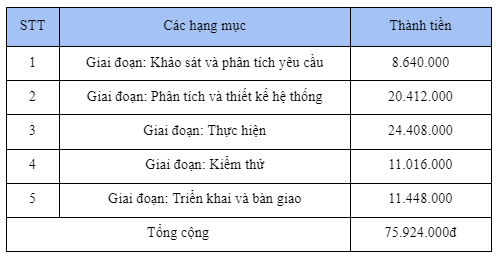
\includegraphics[width=15cm]{ChiPhi9.png}
\vspace{0.5cm}

\subsubsection{Chi phí nguyên vật liệu}
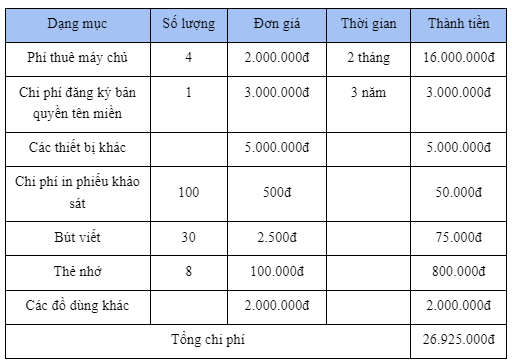
\includegraphics[width=15cm]{ChiPhi10.png}
\vspace{0.5cm}

\subsubsection{Chi phí cơ sở vật chất}
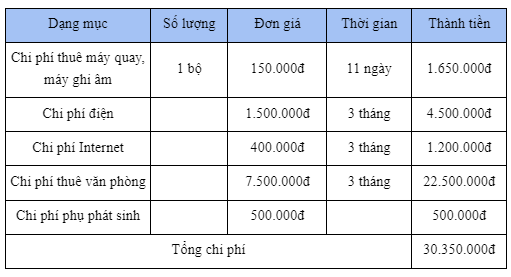
\includegraphics[width=15cm]{ChiPhi11.png}
\vspace{0.5cm}

\subsubsection{Các chi phí phát sinh}
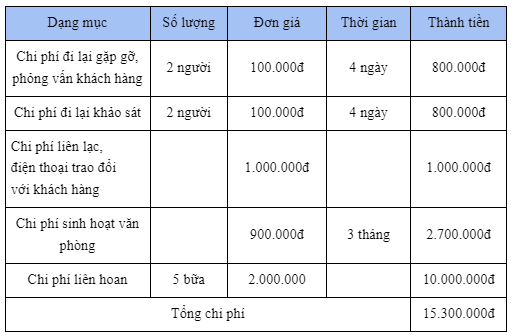
\includegraphics[width=15cm]{ChiPhi12.png}
\vspace{0.5cm}

\subsubsection{Tổng chi phí cho dự án}
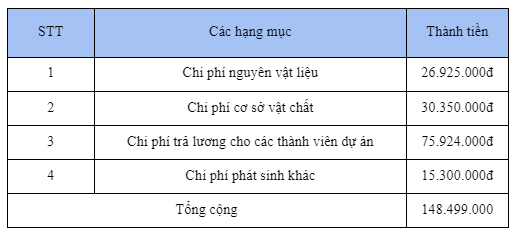
\includegraphics[width=15cm]{ChiPhi13.png}
\par
\begin{adjustwidth}{1cm}{0.5cm} % Lùi 2cm cả bên trái và bên phải
  - Đây là tổng chi phí dự đoán cho dự án xây dựng website bán quần áo trong khoảng ( 142.500.000 - 157.500.000) như dự đoán ban đầu sai lệch khoảng 5\% với kinh phí 150.000.000đ ta có thể kiểm soát được. 
\end{adjustwidth}
\hspace{1cm}

\subsection{Quản lý chất lượng}
\begin{itemize}[label=-, leftmargin=1cm]
    \item Mục đích của quản lý chất lượng :
    \begin{itemize}[label=+, leftmargin=1cm]
        \item Xác định chất lượng sản phẩm thỏa mãn được khách hành không.
        \item Giám sát đánh giá, kịp thời phát hiện sai sót từ đó có kế hoạch khắc phục.
        \item Phạm vi thực hiện.
        \item Được tiến hành ở từng giai đoạn của dự án.
        \item Cách nắm bắt chất lượng.
        \item Đội ngũ DA phải có quan hệ tốt với khách hàng.
        \item Khách hàng là người cuối cùng đánh giá chất lượng dự án. Nhiều dự án thất bại do chỉ chú tâm đến kỹ thuật, mà không quan tâm đến mong đợi của khách hàng.
    \end{itemize}
\end{itemize}

\subsubsection{Các tiêu chuẩn thước đo của phần mềm}
\begin{itemize}[label=-, leftmargin=1cm]
    \item Tính khả dụng của giao diện: Đảm bảo sự đầy đủ và dễ dàng cho người dùng. Giao diện thân thiện, đơn giản và dễ sử dụng với người dùng. Các chức năng của ứng dụng phải đáp ứng đủ được các yêu cầu của khách hàng về quản lý thư viện. 
    \item Tính toàn vẹn của dữ liệu: Đảm bảo dữ liệu đồng bộ, dữ liệu không bị thay đổi hay mất mát, đặc biệt trong xử lý các giao dịch trong hệ thống. Dữ liệu phải đảm bảo được sự toàn vẹn khi được người dùng tiến hành cập nhật.
    \item Tính an toàn bảo mật: Coi trọng tính bảo mật, đảm bảo tính an toàn bảo mật dữ liệu. Ứng dụng phải được lập trình theo mô hình MVC. Mỗi phương thức trong ứng dụng không vượt quá 35-40 dòng code. Ứng dụng phải được chia thành nhiều module riêng biệt theo từng chức năng và dễ dàng tích hợp được với nhau.
    \item Tính ổn định của ứng dụng: Ứng dụng chạy ổn định, ko bị lỗi khi hệ thống và phần mềm xảy ra một số thay đổi. Chương trình gọn nhẹ, ổn định và có khả năng tương thích với nhiều nền tảng hệ điều hành khác nhau. Ứng dụng có khả năng được bảo trì, sửa đổi một cách dễ dàng.
    \item Tính bảo mật: Ứng dụng phải có cơ chế bảo mật tốt, có khả năng tránh được các vụ tấn công thông thường.
\end{itemize}

\subsubsection{Các hình thức kiểm thử có thể dùng}
\begin{itemize}[label=-, leftmargin=1cm]
    \item Kiểm thử chức năng định kì: Các chức năng sẽ được kiểm tra định kỳ để đảm bảo trang web hoạt động trơn tru và không phát sinh lỗi trong quá trình hoạt động. 
    \item Kiểm tra code: Lập trình viên có kinh nghiệm kiểm tra code đột xuất để xem có tuân thủ theo đúng chuẩn mô hình MVC hay không.
    \item Kiểm thử bởi khách hàng: Đưa mẫu thiết kế cho khách hàng để thăm dò phản ứng và lấy ý kiến của khách hàng về giao diện của ứng dụng. Kiểm tra các chức năng của ứng dụng xem đã phù hợp với các yêu cầu của khách hàng hay không dựa trên các giả thiết từ phía khách hàng và tập dữ liệu mẫu.
    \item Kiểm tra tính toàn vẹn của dữ liệu: Dữ liệu của ứng dụng sẽ được kiểm tra tính toàn vẹn dựa theo tập hợp những dữ liệu.
\end{itemize}

\subsubsection{Các bên quản lý chất lượng}
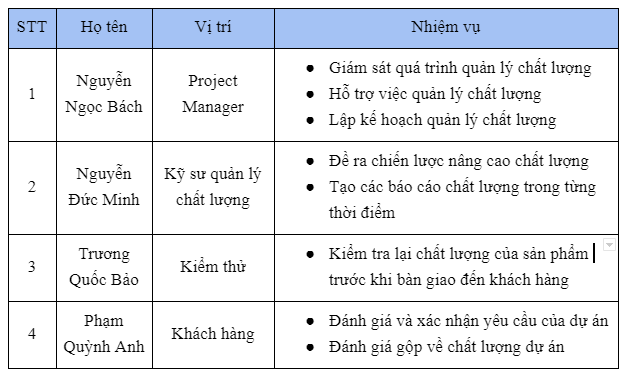
\includegraphics[width=15cm]{II_5_3.png}
\vspace{0.5cm}

\subsubsection{Lập kế hoạch quản lý chất lượng}
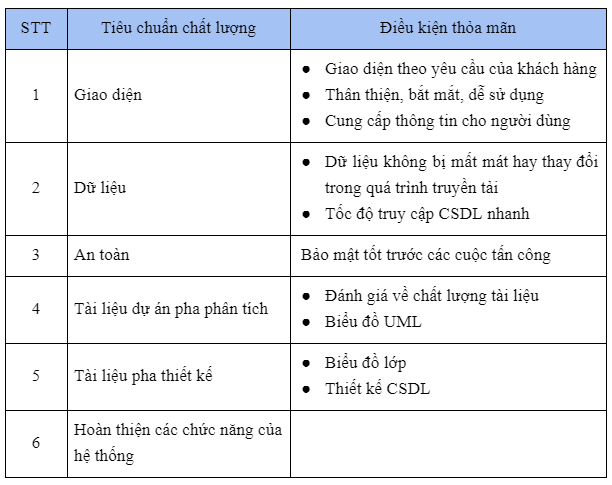
\includegraphics[width=15cm]{II_5_4.png}

\subsubsection{Kiểm soát chất lượng}
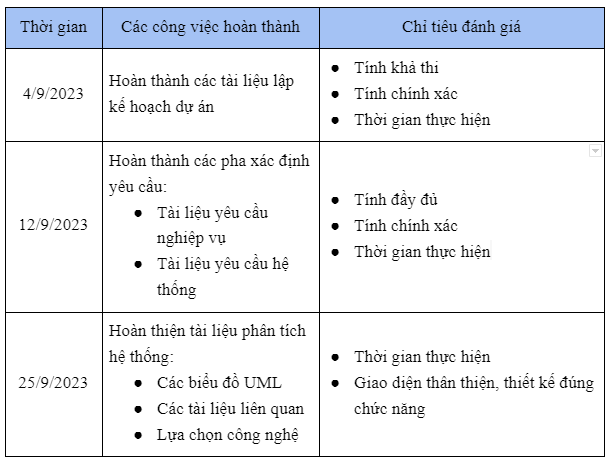
\includegraphics[width=15cm]{II_5_5_1.png}
\par
\hspace{-0.6cm}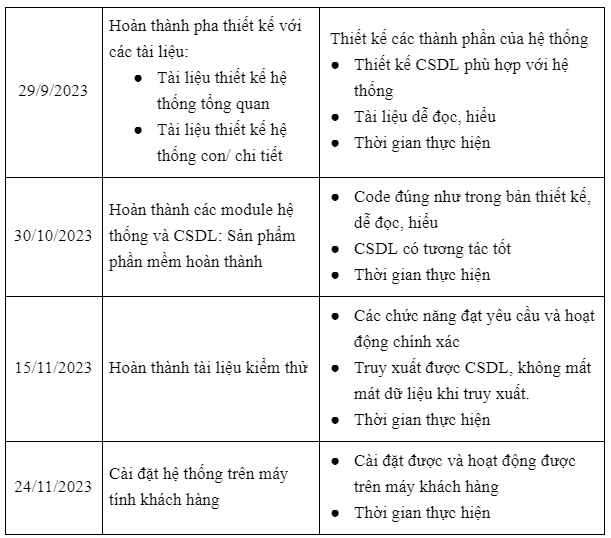
\includegraphics[width=15cm]{II_5_5_2.png}
\vspace{0.5cm}

\subsection{Quản lý nguồn nhân lực}
\subsubsection{Các vị trí trong quản lý dự án}
\includegraphics[width=15cm]{II_6_1_1.png}
\par
\hspace{-0.6cm}\includegraphics[width=15cm]{II_6_1_2.png}
\vspace{0.5cm}

\subsubsection{Danh sách các cá nhân tham gia dự án}
\includegraphics[width=15cm]{II_6_2.png}
\vspace{0.5cm}

\subsubsection{Danh sách các cá nhân tham gia dự án}
\includegraphics[width=15cm]{II_6_3_1.png}
\par
\hspace{-0.6cm}\includegraphics[width=15cm]{II_6_3_2.png}
\vspace{0.5cm}

\subsubsection{Sơ đồ tổ chức}
\includegraphics[width=15cm]{II_6_4.png}
\vspace{0.5cm}

\subsubsection{Phân chia công việc}
\hspace{1cm}\textbf{Phân chia giữa các nhóm \\}
\includegraphics[width=15cm]{II_6_5_1.png}
\begin{itemize}[label=, leftmargin=1cm]
    \item Chú thích:
    \begin{itemize}[label=1, leftmargin=1cm]
        \item A (Approval): Thông qua, phê chuẩn.
        \item L (Leader): Nhóm trưởng.
        \item S (Secondary): Chịu trách nhiệm thay nhóm trưởng nếu nhóm trưởng vắng mặt.
        \item C (Contributor): Cộng tác viên.
        \item R (Reviewer): Người kiểm tra lại.
    \end{itemize}
\end{itemize}
\vspace{0.5cm}
\hspace{1cm}\textbf{Phân chia chi tiết \\}
\includegraphics[width=15cm]{II_6_5_2.png}
\par
\hspace{-0.6cm}\includegraphics[width=15cm]{II_6_5_3.png}
\par
\hspace{-0.6cm}\includegraphics[width=15cm]{II_6_5_4.png}
\vspace{0.5cm}

\subsection{Quản lý rủi ro}
\subsubsection{Quá trình quản lý rủi ro trong khảo sát thực hiện dự án}
\includegraphics[width=10cm]{II_7_1.png}
\vspace{0.5cm}

\subsubsection{Các lĩnh vực xảy ra rủi ro}
\includegraphics[width=12cm]{II_7_2.png}
\vspace{0.5cm}

\subsubsection{Xác định rủi ro}
\includegraphics[width=15cm]{II_7_3_1.png}
\par
\hspace{-0.6cm}\includegraphics[width=15cm]{II_7_3_2.png}
\vspace{0.5cm}
\subsubsection{Phân tích mức độ rủi ro}
\hspace{-2cm}\includegraphics[width=19cm]{II_7_4_1.png}
\par
\hspace{-2.6cm}\includegraphics[width=19cm]{II_7_4_2.png}
\par
\hspace{-2.6cm}\includegraphics[width=19cm]{II_7_4_3.png}
\par
\hspace{-2.6cm}\includegraphics[width=19cm]{II_7_4_4.png}
\vspace{0.5cm}

\subsubsection{Kế hoạch phòng ngừa rủi ro}
\includegraphics[width=15cm]{II_7_5_1.png}
\par
\hspace{-0.6cm}\includegraphics[width=15cm]{II_7_5_2.png}
\par
\hspace{-0.6cm}\includegraphics[width=15cm]{II_7_5_3.png}
\vspace{0.5cm}

\subsubsection{Rủi ro gặp phải}
\hspace{1cm}Trong lúc làm dự án, đã có sự cố xảy ra khi bạn Bách đã không hoàn thành tiến độ công việc được giao. Mã công việc “3.2.3 Tối ưu hóa giao diện cho tính responsive và tương thích”. Thời gian từ 12/10/2023 đến 17/10/2023. Do đó, bạn Bách phải viết biên bản không hoàn thành công việc và nộp lên trên. (đây là biên bản, giải thích). Đây là biểu đồ thời gian cho phần công việc không hoàn thành (show biểu đồ). Vì công việc “3.2.3 Tối ưu hóa giao diện cho tính responsive và tương thích” không bị ảnh hưởng đến các tiến trình sau nên giám đốc dự án quyết định cho Bách làm lại với thời gian 4 ngày từ 18/10/2023 - 23/10/2023 và tiến hành xử phạt mức độ nhẹ.
\begin{center}
\begin{adjustbox}{max width=16cm}
\hspace{-2cm}
\begin{tikzpicture}
  \node[inner sep=0pt] (image1) {\includegraphics{bien_ban_khong_hoan_thanh.png}};
  \draw[line width=2pt, color=black] (image1.north west) rectangle (image1.south east);
\end{tikzpicture}
\end{adjustbox}
\end{center}


\newpage
\subsection{Các loại biên bản}
\subsubsection{Biên bản cuộc họp}
\begin{center}
\begin{adjustbox}{max width=16cm}
\hspace{-1.5cm}
\begin{tikzpicture}
  \node[inner sep=0pt] (image1) {\includegraphics{bien_ban_cuoc_hop_1.png}};
  \draw[line width=2pt, color=black] (image1.north west) rectangle (image1.south east);
\end{tikzpicture}
\end{adjustbox}

\begin{adjustbox}{max width=16cm}
\hspace{-1.5cm}
\begin{tikzpicture}
  \node[inner sep=0pt] (image2) {\includegraphics{bien_ban_cuoc_hop_2.png}};
  \draw[line width=2pt, color=black] (image2.north west) rectangle (image2.south east);
\end{tikzpicture}
\end{adjustbox}

\begin{adjustbox}{max width=16cm}
\hspace{-1.5cm}
\begin{tikzpicture}
  \node[inner sep=0pt] (image3) {\includegraphics{bien_ban_cuoc_hop_3.png}};
  \draw[line width=2pt, color=black] (image3.north west) rectangle (image3.south east);
\end{tikzpicture}
\end{adjustbox}
\end{center}
\newpage

\subsubsection{Biên bản không hoàn thành công việc đúng yêu cầu}
\begin{center}
\begin{adjustbox}{max width=16cm}
\hspace{-1.5cm}
\begin{tikzpicture}
  \node[inner sep=0pt] (image1) {\includegraphics{bien_ban_khong_hoan_thanh.png}};
  \draw[line width=2pt, color=black] (image1.north west) rectangle (image1.south east);
\end{tikzpicture}
\end{adjustbox}
\end{center}
\newpage

\subsubsection{Biên bản bàn giao sản phẩm}
\begin{center}
\begin{adjustbox}{max width=16cm}
\begin{tikzpicture}
  \node[inner sep=0pt] (image1) {\includegraphics{bien-ban-giao-nhan.jpg}};
  \draw[line width=2pt, color=black] (image1.north west) rectangle (image1.south east);
\end{tikzpicture}
\end{adjustbox}
\end{center}

\newpage

\part{CHUYỂN GIAO}
\begin{tabularx}{\textwidth}{|>{\raggedright\arraybackslash}X|}
    \hline
    {\cellcolor[HTML]{6D9EEB}\textbf{\rule{0pt}{1cm}\makecell{\ BIÊN BẢN BÀN GIAO SẢN PHẨM \vspace{0.4cm}}}} \\
    \hline
    \multicolumn{1}{|p{\dimexpr\linewidth-0.5cm-2\tabcolsep}|}{%
    \begin{center}
        CỘNG HÒA XÃ HỘI CHỦ NGHĨA VIỆT NAM \\
        Độc lập - Tự do - Hạnh phúc \\
        \vspace{0.6cm}
        \textbf{BIÊN BẢN BÀN GIAO SẢN PHẨM \\}
        Giữa: Nhóm 1 với Công Ty TNHH MTV Hồng Diệp
    \end{center}
    \vspace{0.3cm}
    \begin{itemize}[label=, leftmargin=0.5cm]
        \item \hspace{1cm}Hôm nay ngày 25 tháng 11 năm 2023 tại 175 Tây Sơn Hà Nội đã tiến hành cuộc họp bàn giao sản phẩm giữa dự án của Nhóm 1 (bên giao) và bà Trần Hồng Diệp (bên nhận) thực hiện theo biên bản làm việc giữa 2 bên ngày 25/11/2023.
        \item \textbf{I/ THÀNH PHẦN THAM DỰ}
        \item 1/ Bên giao
        \item \begin{minipage}{0.35\textwidth}
            - Ông: Nguyễn Ngọc Bách \vspace{0.1cm}
            \end{minipage}%
            \begin{minipage}{0.55\textwidth}
            \raggedright
            Chức vụ: Giám đốc dự án.
            \end{minipage}
        \item 2/ Bên nhận
        \item \begin{minipage}{0.35\textwidth}
            - Bà: Trần Hồng Diệp \vspace{0.5cm}
            \end{minipage}%
            \begin{minipage}{0.55\textwidth}
            \raggedright
            Chức vụ: Đại diện Công Ty TNHH MTV Hồng Diệp.
            \end{minipage}
        \item \textbf{II/ NỘI DUNG BÀN GIAO}
        \item - Bên chủ đầu tư đã tiến hành bàn giao tài sản cho bên thiết kế theo biểu thống kê sau:
        \item \begin{center}
            \textbf{Bản thống kê tài sản bàn giao}
            \end{center}
        \item 
            \begin{tabular*}{\linewidth}{|>       {\centering\arraybackslash}p{1cm}|>{\centering\arraybackslash}p{3cm}|>
            {\centering\arraybackslash}p{1cm}|>{\centering\arraybackslash}p{3.2cm}|>{\centering\arraybackslash}p{3.2cm}|}
            \hline
            \cellcolor[HTML]{C6D9F1}\rule{0pt}{1cm}\textbf{STT \vspace{0.1cm}} & \cellcolor[HTML]{C6D9F1}\textbf{Tên sản phẩm} & \cellcolor[HTML]{C6D9F1}\textbf{SL} & \cellcolor[HTML]{C6D9F1}\textbf{Đơn giá} & \cellcolor[HTML]{C6D9F1}\textbf{Thành tiền} \\
            \hline
            \rule{0pt}{1cm}1 & Nền tảng bán vé trực tuyến TicketFusion \vspace{0.5cm} & 1 & 150.000.000VNĐ & 150.000.000VNĐ \\
            \hline
            \end{tabular*}
    \end{itemize}
    } \\
    \vspace{0.05cm} \\
    \hline
\end{tabularx}

\begin{tabularx}{\textwidth}{|>{\raggedright\arraybackslash}X|}
    \hline
    \multicolumn{1}{|p{\dimexpr\linewidth-0.5cm-2\tabcolsep}|}{%
    \begin{itemize}[label=, leftmargin=0.5cm]
        \item \textbf{Tổng giá trị:}
            \begin{itemize}[label=+, leftmargin=0.5cm]
                \item Bằng số: 150.000.000 VNĐ.
                \item Bằng chữ: Một trăm triệu đồng chẵn (Đã thanh toán).
            \end{itemize}
        \item \textbf{Bên thiết kế đã tiến hành bàn giao sản phẩm cho bên nhà đầu tư:}
        \begin{itemize}[label=+, leftmargin=0.5cm]
                \item 01 hệ thống Hệ Thống mua bán vé sự kiện với đầy đủ chức năng và hoạt động bình thường, hệ thống trên nền tảng website.
                \item Quá trình bảo trì và trách nhiệm của từng bên sẽ được tiến hành theo biên bản hợp đồng đã ký vào 25/11/2023.
            \end{itemize}
        \item Biên bản này : Bên giao giữ 1 bản, bên nhận giữ 1 bản.
        \item \begin{minipage}{0.4\textwidth}
                \begin{center}
                    CHỮ KÝ BÊN GIAO \\
                    (Ký và ghi gõ họ tên)\\
                    \includegraphics[width=6cm]{signature1.png}\\ 
                    Nguyễn Ngọc Bách
                \end{center}
            \end{minipage}%
            \begin{minipage}{0.6\textwidth}
                \begin{center}
                    CHỮ KÝ BÊN NHẬN \\
                    (Ký và ghi gõ họ tên)\\
                    \includegraphics[width=6cm]{signature2.png} \\ 
                    Trần Hồng Diệp
                \end{center}
            \end{minipage}
    \end{itemize}
    } \\
    \vspace{0.5cm} \\
    \hline
\end{tabularx}


\newpage
\part{KẾT LUẬN}
\hspace{1cm}Sau một thời gian nhóm bắt tay vào nghiên cứu cùng với sự giúp đỡ của cô Trần Hồng Diệp, nhóm chúng tôi đã hoàn thành đề tài “Xây dựng Website mua bán vé sự kiện”. Chúng tôi gửi đến cô lời cảm ơn trân trọng nhất. Qua đây bản thân tôi cũng như các thành viên trong nhóm đã học hỏi được rất nhiều điều về công việc, trang bị cho các thành viên các kiến thức cơ bản về thiết kế, quản lý, kế hoạch quản lý thời gian, chi phí và điều hành các dự án CNTT cùng một số kiến thức, kỹ năng để tổ chức và tham gia đấu thầu dự án CNTT. Học phần cũng rèn luyện cho sinh viên kỹ năng làm việc theo nhóm và kỹ năng lãnh đạo nhóm dự án. Tuy nhiên trong quá trình phân tích, thiết kế và xây dựng hệ thống, do thời gian có hạn cũng như kinh nghiệm của bản thân còn hạn chế nên chắc chắn báo cáo không tránh khỏi những thiếu sót và những chỗ xử lý vấn đề chưa được tối ưu. Chúng tôi rất mong nhận được những nhận xét, đánh giá từ phía các thầy cô, đặc biệt của giảng viên hướng dẫn và giảng dạy môn học Quản lý dự án Công nghệ thông tin. 

\end{document}

